
%Este archivo no tiene contenido, mas allá de configuraciones y\o definiciones.
%todo el contenido se encuentra en los archivos secundarios que son importados por este.

\documentclass[twoside,letterpaper]{article}


%\\\\\\\\\\\\\\\\\\\\\\\\\\\
%Packages en uso

%Idiomas diccionario
\usepackage[english, spanish]{babel}
%\usepackage[english]{babel}

\usepackage[utf8x]{inputenc}
%\usepackage[latin1]{inputenc} 
%\usepackage[ansinew]{inputenc}
\usepackage{ucs}




%\usepackage[margin=1cm, paperwidth=21.0cm, paperheight=29.6cm]{geometry}



\usepackage[T1]{fontenc} 
\usepackage{graphicx}
\usepackage{float}
\usepackage{longtable}
%\usepackage{floatflt}
\usepackage{fancyhdr}
\usepackage{hyperref}
%\usepackage{url}
\usepackage{amsfonts}
\usepackage{amssymb}
\usepackage{textcomp}
%\usepackage[symbol]{footmisc}
%\usepackage{pst-circ}
%\usepackage{epsfig}
%\usepackage{xkeyval}
\usepackage{tabularx}
\usepackage{booktabs}


%\usepackage{color}
\usepackage[usenames,dvipsnames]{color}


%\usepackage{minted}
\usepackage{latexsym}
\usepackage{colortbl}
%\usepackage{pdfpages}
\usepackage{wrapfig}

%\usepackage{listings}
\usepackage{listingsutf8}
%\usepackage{mips}
\usepackage{appendix}
\usepackage{needspace}
\usepackage{ifplatform}
\usepackage{ifthen}
\usepackage{amsmath}


%\\\\\\\\\\\\\\\\\\\\\\\\\\\
% FOR GNUPLOT
%\usepackage{tikz}

%\usepackage[miktex]{gnuplottex}
%\usepackage{gnuplot-lua-tikz}
%\usepackage{mathpazo}
%\\\\\\\\\\\\\\\\\\\\\\\\\\\


%\\\\\\\\\\\\\\\\\\\\\\\\\\\
% FOR FIGURE CAPTION COLORS

\usepackage{caption}
\usepackage[svgnames]{xcolor}

%\\\\\\\\\\\\\\\\\\\\\\\\\\\


%\\\\\\\\\\\\\\\\\\\\\\\\\\\
% FOR EQUATION CAPTION FORMAT, COLORS AND OTHERS

\usepackage{mathtools}

%\\\\\\\\\\\\\\\\\\\\\\\\\\\


%\\\\\\\\\\\\\\\\\\\\\\\\\\\
% TABLES

\usepackage{makecell, multirow, tabularx}
    \newcolumntype{L}{>{\raggedright\arraybackslash}X}
    \renewcommand\theadfont{\normalsize\bfseries\color{white}}
\usepackage{hhline}
\usepackage{setspace}

%\\\\\\\\\\\\\\\\\\\\\\\\\\\


%\\\\\\\\\\\\\\\\\\\\\\\\\\\
% UNITS

\usepackage{siunitx}

\sisetup{output-exponent-marker=\ensuremath{\mathrm{e}}}

%\\\\\\\\\\\\\\\\\\\\\\\\\\\



%\\\\\\\\\\\\\\\\\\\\\\\\\\\
%!!!!!!!!!!!!!!!!!!!!!!!!! DETECCION DE PLATAFORMA !!!!!!!!!!!!!!!!!!!!!!!!!!!!!!!!!
%Permite que sea compilado tanto en windows como en *IX sin cambio alguno.
\newboolean{IsWindows}
\ifwindows
\setboolean{IsWindows}{true}
\else
\setboolean{IsWindows}{false}
\fi
%\\\\\\\\\\\\\\\\\\\\\\\\\\\
%!!!!!!!!!!!!!!!!!!!!!!!!!!!!!!!!!!!!!!!!!!!!!!!!!!!!!!!!!!!!!!!!!!!!!!!!!!!!!!!!!!!!

%\\\\\\\\\\\\\\\\\\\\\\\\\\\
%Idiomas
\hyphenrules{spanish}
%\\\\\\\\\\\\\\\\\\\\\\\\\\\


%\\\\\\\\\\\\\\\\\\\\\\\\\\\
%Comandos personalizados

\newcommand{\titulo}{Trabajo práctico N\textdegree \hspace{1pt} 1A}
\newcommand{\titulolargo}{Análisis de fuente lineal}
\newcommand{\materia}{Circuitos electrónicos II - 66.10}
\newcommand{\fiuba}{Facultad de Ingeniería - UBA}
\newcommand{\cuatrimestre}{1\textsuperscript{er} c. 2019} %\sptext{do} $2^{do}$


\newcommand{\autorA}{\textsc{Irusta} Pablo}
\newcommand{\padronA}{80171}
\newcommand{\mailA}{\weblink{mailto:pabirus@gmail.com}{pabirus@gmail.com}}


\newcommand{\autorB}{\textsc{Luna} Diego}
\newcommand{\padronB}{75451}
\newcommand{\mailB}{\weblink{mailto:diegorluna@gmail.com}{diegorluna@gmail.com}} 
 
\newcommand{\autorC}{\textsc{Niero} Adrián}
\newcommand{\padronC}{80533}
\newcommand{\mailC}{\weblink{mailto:adrianniero@gmail.com}{adrianniero@gmail.com}} 
 
\newcommand{\autorD}{\textsc{Romero} Daniel}
\newcommand{\padronD}{69456}
\newcommand{\mailD}{\weblink{mailto:danielosrom@gmail.com}{danielosrom@gmail.com}}  
 
 
 
\newcommand{\docenteA}{Ing. \textsc{Bertuccio} José Alberto}
\newcommand{\docenteB}{Ing. \textsc{Acquaticci} Fabián}
\newcommand{\docenteC}{Ing. \textsc{Marchi} Edgardo }
\newcommand{\docenteD}{Ing. \textsc{Bulacio} Matías}
\newcommand{\docenteE}{Ing. \textsc{D’Angiolo} Federico}
\newcommand{\docenteF}{Ing. \textsc{Gamez} Pablo}


\newcommand{\thedate}{13 de abril de 2019}


\newcommand{\HRule}{\rule{\linewidth}{0.3mm}}

%\\\\\\\\\\\\\\\\\\\\\\\\\\\


%\\\\\\\\\\\\\\\\\\\\\\\\\\\
%Título,  autor del documento y fecha
\title{\titulo}
\author{\autorB}
\date{\thedate}
%\\\\\\\\\\\\\\\\\\\\\\\\\\\


%\\\\\\\\\\\\\\\\\\\\\\\\\\\
\setcounter{secnumdepth}{5}
\setcounter{tocdepth}{5}
%\\\\\\\\\\\\\\\\\\\\\\\\\\\


%\\\\\\\\\\\\\\\\\\\\\\\\\\\
%suppress widows and orphans
\widowpenalty=9999
\clubpenalty=9999
%\\\\\\\\\\\\\\\\\\\\\\\\\\\


%\\\\\\\\\\\\\\\\\\\\\\\\\\\
%equation numbers to subsection level
%\numberwithin{equation}{subsection}
\numberwithin{equation}{section}
%\\\\\\\\\\\\\\\\\\\\\\\\\\\


%\\\\\\\\\\\\\\\\\\\\\\\\\\\
%equation numbers to subsection level
%\numberwithin{table}{subsection}
\numberwithin{table}{section}
%\\\\\\\\\\\\\\\\\\\\\\\\\\\



%\\\\\\\\\\\\\\\\\\\\\\\\\\\
%figure numbers to subsection level
%\renewcommand{\thefigure}{\thesubsection.\arabic{figure}}
\renewcommand{\thefigure}{\thesection.\arabic{figure}}
%\\\\\\\\\\\\\\\\\\\\\\\\\\\

%\setlength{\arrayrulewidth}{0.6pt}


%\\\\\\\\\\\\\\\\\\\\\\\\\\\
\newcolumntype{z}[1]{%
>{\centering\hspace{0pt}}p{#1}}%

\newcolumntype{y}[1]{%
>{\raggedleft\hspace{0pt}}p{#1}}% 

\newcolumntype{x}[1]{%
>{\raggedright\hspace{0pt}}p{#1}}% 

\newcolumntype{w}[1]{%
>{\centering\hspace{0pt}}m{#1}}%

\newcolumntype{v}[1]{%
>{\raggedleft\hspace{0pt}}m{#1}}% 

\newcolumntype{u}[1]{%
>{\raggedright\hspace{0pt}}m{#1}}% 


\newcommand{\tn}{\tabularnewline}
%\\\\\\\\\\\\\\\\\\\\\\\\\\\




%\\\\\\\\\\\\\\\\\\\\\\\\\\\
% Generales
\newcommand{\quotemarks}[1]{``#1''}
\newcommand{\simplequotemarks}[1]{`#1'}
%\\\\\\\\\\\\\\\\\\\\\\\\\\\


%\\\\\\\\\\\\\\\\\\\\\\\\\\\
% Símbolos de las unidades

\newcommand{\volt}[1]{\mbox{#1 V}}
\newcommand{\milivolt}[1]{\mbox{#1 mV}}
\newcommand{\hertz}[1]{\mbox{#1 Hz}}
\newcommand{\kilohertz}[1]{\mbox{#1 kHz}}
\newcommand{\megahertz}[1]{\mbox{#1 MHz}}
\newcommand{\farad}[1]{\mbox{#1 F}}
\newcommand{\nanofarad}[1]{\mbox{#1 nF}}
\newcommand{\microfarad}[1]{\mbox{#1 $\mu$F}}
\newcommand{\picofarad}[1]{\mbox{#1 pF}}
\newcommand{\fentofarad}[1]{\mbox{#1 fF}}
\newcommand{\ohm}[1]{\mbox{#1 $\Omega$}}
\newcommand{\miliohm}[1]{\mbox{#1 m$\Omega$}}
\newcommand{\kiloohm}[1]{\mbox{#1 k$\Omega$}}
\newcommand{\megaohm}[1]{\mbox{#1 M$\Omega$}}
\newcommand{\amper}[1]{\mbox{#1 A}}
\newcommand{\miliamper}[1]{\mbox{#1 mA}}
\newcommand{\microamper}[1]{\mbox{#1 $\mu$A}}
\newcommand{\picoamper}[1]{\mbox{#1 pA}}
\newcommand{\fentoamper}[1]{\mbox{#1 fA}}
\newcommand{\s}[1]{\mbox{#1 s}}
\newcommand{\milis}[1]{\mbox{#1 ms}}
\newcommand{\micros}[1]{\mbox{#1 $\mu$s}}
\newcommand{\nanos}[1]{\mbox{#1 ns}}
\newcommand{\miliamperporvolt}[1]{ \mbox{#1 $\frac{mA}{V}$}}
\newcommand{\miliamperporvoltcuad}[1]{ \mbox{#1 $\frac{mA}{V^2}$}}
\newcommand{\decibel}[1]{\mbox{#1 dB}}
\newcommand{\decibeli}[1]{\mbox{#1 dBi}}

\newcommand{\spice}{\mbox{\textit{\textbf{SPICE}}}}
\newcommand{\schematic}{\mbox{\textit{\textbf{SCHEMATIC}}}}

% Nombres de las unidades
\newcommand{\Metro}{\mbox{metro}}
\newcommand{\Volt}{\mbox{Volt}}
\newcommand{\Amper}{\mbox{Ampere}}
\newcommand{\Farad}{\mbox{Farad}}
%\\\\\\\\\\\\\\\\\\\\\\\\\\\

%\\\\\\\\\\\\\\\\\\\\\\\\\\\
% Dispositivos

\newcommand{\mosfet}{\mbox{\textbf{MOSFET}}}
\newcommand{\nmosfet}{\mbox{\textbf{NMOSFET}}}
\newcommand{\bjtnpn}{\mbox{\textbf{BJT NPN}}}
\newcommand{\bjtpnp}{\mbox{\textbf{BJT PNP}}}

%\\\\\\\\\\\\\\\\\\\\\\\\\\\

%\\\\\\\\\\\\\\\\\\\\\\\\\\\
% Plataformas

\newcommand{\platformhost}{\textbf{x86(\_64)\textbackslash Linux}}
\newcommand{\platformguest}{\textbf{pmax\textbackslash NetBSD}}

\newcommand{\oshost}{\textbf{Linux}}
\newcommand{\osguest}{\textbf{NetBSD}}

\newcommand{\MIPS}{\textbf{MIPS32}}
%\\\\\\\\\\\\\\\\\\\\\\\\\\\


%\\\\\\\\\\\\\\\\\\\\\\\\\\\
% Programación

\newcommand{\GNU}{\textbf{GNU}}

\newcommand{\GCC}{\textbf{GCC}}

\newcommand{\GDB}{\textbf{GDB}}

\newcommand{\GXEMUL}{\textbf{GXemul}}

\newcommand{\langc}{\textbf{\quotemarks{C}}}

\newcommand{\langass}{\textbf{assembly}}

\newcommand{\langmipsass}{\textbf{MIPS32 assembly}}

\newcommand{\make}{\textbf{make}}
%\\\\\\\\\\\\\\\\\\\\\\\\\\\


%\\\\\\\\\\\\\\\\\\\\\\\\\\\
% Archivos

\newcommand{\quotefile}[1]{\textit{\quotemarks{#1}}}

\newcommand{\filebox}[2]{%

\begin{tabular}{l}

\multicolumn{1}{>{\columncolor{#2}}l}{#1} 
	
\end{tabular}

}%
%\\\\\\\\\\\\\\\\\\\\\\\\\\\



%\\\\\\\\\\\\\\\\\\\\\\\\\\\
% Math
\newcommand{\Reales}{\mathbb{R}}
\newcommand{\Complejos}{\mathbb{C}}
\newcommand{\numnorm}[1]{\left|#1\right|}
\newcommand{\vectornorm}[1]{\left|\left|#1\right|\right|}
%\\\\\\\\\\\\\\\\\\\\\\\\\\\


%\\\\\\\\\\\\\\\\\\\\\\\\\\\
% Counters
\newcommand{\resetallcounters}{%
\setcounter{figure}{0}
\setcounter{equation}{0}
\setcounter{table}{0}
}%
%\\\\\\\\\\\\\\\\\\\\\\\\\\\



%\\\\\\\\\\\\\\\\\\\\\\\\\\\
% Definiciones de colores.
\definecolor{Deepblue}{rgb}{0.00,0.00,0.70}
\definecolor{Deepgreen}{rgb}{0.09,0.45,0.20}
\definecolor{Darkgreen}{RGB}{0, 128, 0}
\definecolor{Purple}{rgb}{1,0,1}
\definecolor{Deeppurple}{rgb}{0.2,0,1}
\definecolor{Gray}{rgb}{0.3,0.3,0.3}
\definecolor{Lightblue}{rgb}{0.60, 0.80, 1.00}
\definecolor{Lightyellow}{rgb}{1.00,1.00,0.60}
\definecolor{LightButter}{rgb}{0.98,0.91,0.31}
\definecolor{LightOrange}{rgb}{0.98,0.68,0.24}
\definecolor{LightChocolate}{rgb}{0.91,0.72,0.43}
\definecolor{LightChameleon}{rgb}{0.54,0.88,0.20}
\definecolor{LightSkyBlue}{rgb}{0.45,0.62,0.81}
\definecolor{LightPlum}{rgb}{0.68,0.50,0.66}
\definecolor{LightScarletRed}{rgb}{0.93,0.16,0.16}
\definecolor{Butter}{rgb}{0.93,0.86,0.25}
\definecolor{Orange}{rgb}{0.96,0.47,0.00}
\definecolor{Chocolate}{rgb}{0.75,0.49,0.07}
\definecolor{Chameleon}{rgb}{0.45,0.82,0.09}
\definecolor{SkyBlue}{rgb}{0.20,0.39,0.64}
\definecolor{Plum}{rgb}{0.46,0.31,0.48}
\definecolor{ScarletRed}{rgb}{0.80,0.00,0.00}
\definecolor{DarkButter}{rgb}{0.77,0.62,0.00}
\definecolor{DarkOrange}{rgb}{0.80,0.36,0.00}
\definecolor{DarkChocolate}{rgb}{0.56,0.35,0.01}
\definecolor{DarkChameleon}{rgb}{0.30,0.60,0.02}
\definecolor{DarkSkyBlue}{rgb}{0.12,0.29,0.53}
\definecolor{DarkPlum}{rgb}{0.36,0.21,0.40}
\definecolor{DarkScarletRed}{rgb}{0.64,0.00,0.00}
\definecolor{Aluminium1}{rgb}{0.93,0.93,0.92}
\definecolor{Aluminium2}{rgb}{0.82,0.84,0.81}
\definecolor{Aluminium3}{rgb}{0.73,0.74,0.71}
\definecolor{Aluminium4}{rgb}{0.53,0.54,0.52}
\definecolor{Aluminium5}{rgb}{0.33,0.34,0.32}
\definecolor{Aluminium6}{rgb}{0.18,0.20,0.21}

\definecolor{EQColor}{rgb}{0.00,0.26,0.36} % {0.80,0.36,0.00}
\definecolor{FIGColor}{cmyk}{1,0.00,0.00,0.00}
\definecolor{TABLEColor}{RGB}{0,199,199}



\definecolor{APENDLINKColor}{rgb}{0.96,0.47,0.00}
\definecolor{SECTLINKColor}{rgb}{1.00,0.00,0.00}
\definecolor{FILELINKColor}{rgb}{1.00,0.00,0.00}
\definecolor{INTERNALLINKColor}{rgb}{1.00,0.00,0.00}
\definecolor{WEBLINKColor}{rgb}{0.00,0.00,1.00}
\definecolor{CITELINKColor}{RGB}{141,199,126}
\definecolor{TABLELINKColor}{RGB}{199,199,0}


%\definecolor{EQColor}{rgb}{0.00,0.36,0.80}
%\definecolor{FIGColor}{cmyk}{1,0.00,0.00,0.00}
%\definecolor{TABLEColor}{RGB}{0,199,25}



%\definecolor{APENDLINKColor}{rgb}{0.10,0.47,0.00}
%\definecolor{SECTLINKColor}{rgb}{0.00,0.00,1.00}
%\definecolor{FILELINKColor}{rgb}{0.00,0.00,1.00}
%\definecolor{INTERNALLINKColor}{rgb}{0.00,0.00,1.00}
%\definecolor{WEBLINKColor}{rgb}{0.00,0.00,1.00}
%\definecolor{CITELINKColor}{RGB}{141,199,126}
%\definecolor{TABLELINKColor}{RGB}{199,199,0}


\definecolor{HeadersColor}{RGB}{0,137,182}

%\\\\\\\\\\\\\\\\\\\\\\\\\\\


%\\\\\\\\\\\\\\\\\\\\\\\\\\\
% FOR FIGURE CAPTION COLORS

\DeclareCaptionFont{FIGFont}{\color{FIGColor}}
\captionsetup[figure]{labelfont={FIGFont,bf}}

\newcommand{\figref}[1]{\textcolor{FIGColor}{[\ref{#1}]}}
%\\\\\\\\\\\\\\\\\\\\\\\\\\\


%\\\\\\\\\\\\\\\\\\\\\\\\\\\
% FOR TABLE CAPTION COLORS

\DeclareCaptionFont{TABLEFont}{\color{TABLEColor}}
\captionsetup[table]{labelfont={TABLEFont,bf}}

\newcommand{\tableref}[1]{\textcolor{TABLEColor}{[\ref{#1}]}}


%\captionsetup[table]{style=fortables}
%\captionsetup[figure]{style=forfigures}
%\\\\\\\\\\\\\\\\\\\\\\\\\\\


%\\\\\\\\\\\\\\\\\\\\\\\\\\\
% FOR EQUATION CAPTION FORMAT, COLORS AND OTHERS

\newtagform{brackets2}[\textcolor{EQColor}]{\textcolor{EQColor}(}{\textcolor{EQColor})}
\usetagform{brackets2}

%\\\\\\\\\\\\\\\\\\\\\\\\\\\


%\\\\\\\\\\\\\\\\\\\\\\\\\\\
% FOR EQUATION CAPTION COLORS
%\makeatletter %% Without ams
%\def\@eqnnum{{\normalfont\normalcolor[\theequation]}}
%\makeatother

%But amsmath redefines the numbering of equations, so then you can do:

%\makeatletter %% With ams
%\def\tagform@#1{\maketag@@@{[\ignorespaces#1\unskip\@@italiccorr]}}
%\makeatother 
%\\\\\\\\\\\\\\\\\\\\\\\\\\\


%\\\\\\\\\\\\\\\\\\\\\\\\\\\
% FOR APENDIX REFERENCE

\newcommand{\apendref}[1]{\textcolor{APENDLINKColor}{[\ref{#1}]}}

%\\\\\\\\\\\\\\\\\\\\\\\\\\\


%\\\\\\\\\\\\\\\\\\\\\\\\\\\
% FOR SECTION REFERENCE

\newcommand{\sectref}[1]{\textcolor{SECTLINKColor}{[\ref{#1}]}}

%\\\\\\\\\\\\\\\\\\\\\\\\\\\


%\\\\\\\\\\\\\\\\\\\\\\\\\\\
% WEB LINK

\newcommand{\weblink}[2]{\href{#1}{\textcolor{WEBLINKColor}{#2}}}

%\\\\\\\\\\\\\\\\\\\\\\\\\\\


%\\\\\\\\\\\\\\\\\\\\\\\\\\\
% FILE LINK

\newcommand{\filelink}[2]{\href{#1}{\textcolor{FILELINKColor}{#2}}}

%\\\\\\\\\\\\\\\\\\\\\\\\\\\


%\\\\\\\\\\\\\\\\\\\\\\\\\\\
% CITE LINK
\newcommand{\citelink}[1]{\textcolor{LimeGreen}{\cite{#1}}}

%\\\\\\\\\\\\\\\\\\\\\\\\\\\


\hypersetup{
%	bookmarksnumbered,
%	pdfpagemode={UseOutlines},
%    bookmarks=true,         				% show bookmarks bar?
    unicode=true,          					% non-Latin characters in Acrobat’s bookmarks
    pdftoolbar=true,        				% show Acrobat’s toolbar?
    pdfmenubar=true,        				% show Acrobat’s menu?
%    pdffitwindow=false,    				% window fit to page when opened
%    pdfstartview={FitH},   				% fits the width of the page to the window
    pdftitle={\titulo},   					% title
    pdfauthor={\autorA},    				% author
    pdfsubject={\materia},   				% subject of the document
%    pdfcreator={\LaTeX},   				% creator of the document
%    pdfproducer={Producer},				% producer of the document
    pdfkeywords={TL} {TP}, 					% list of keywords
    pdfnewwindow=true,      				% links in new window
    linktoc=all,							%
    colorlinks=false,  						% false: boxed links; true: colored links	
	linkcolor=INTERNALLINKColor,			% color of internal links
    citecolor=CITELINKColor,    			% color of links to bibliography
    filecolor=FILELINKColor,   	 			% color of file links
    urlcolor=WEBLINKColor,       			% color of external links	
	linkbordercolor=INTERNALLINKColor,		% color of internal links
	citebordercolor=CITELINKColor,			% color of links to bibliography
    filebordercolor=FILELINKColor,    		% color of file links
    urlbordercolor=WEBLINKColor}	       	% color of external links	    
   				
	


%\\\\\\\\\\\\\\\\\\\\\\\\\\\
%Comportamiento de los links a archivos externos.
%\hypersetup{pdfnewwindow=true}
%\\\\\\\\\\\\\\\\\\\\\\\\\\\

%\\\\\\\\\\\\\\\\\\\\\\\\\\\
%Tamaños de la página y margenes

\linespread{1.3}
\oddsidemargin .1cm
\evensidemargin .1cm
\textwidth 16.5cm
\topmargin 0in
\voffset = 0pt
\textheight 21.08cm %8.3in
%\\\\\\\\\\\\\\\\\\\\\\\\\\\



%\pagestyle{fancy}


%\\\\\\\\\\\\\\\\\\\\\\\\\\\
%Encabezado y pie de páginas para todas las páginas normales

\fancypagestyle{allpages}{%

\fancyhf{}  

\renewcommand{\headrulewidth}{0.4pt}
\renewcommand{\footrulewidth}{0.4pt}

%No convierte a mayúscula los nombres de capítulo y sección 
%ni muestra el número.
%\renewcommand{\chaptermark}[1]{}
\renewcommand{\sectionmark}[1]{\markright{##1}{}}
\renewcommand{\subsectionmark}[1]{}
\renewcommand{\subsubsectionmark}[1]{}


\setlength{\headheight}{12pt}

   
%\fancyhf[LOH,REH]{\fiuba}
%\fancyhf[ROH,LEH]{\titulo}

\fancyhf[LH]{\small{\fiuba}}
\fancyhf[CH]{\small{\materia}}
\fancyhf[RH]{\titulo} 

\fancyhf[LOF,REF]{\small{\cuatrimestre}}
\fancyhf[CF]{\small{\rightmark}}
\fancyhf[LEF, ROF]{\textbf{\thepage}} 

}

%\\\\\\\\\\\\\\\\\\\\\\\\\\\


%\\\\\\\\\\\\\\\\\\\\\\\\\\\
%Encabezado y pie de páginas para el índice
\fancypagestyle{indexstyle}{%

\fancyhf{} % clear all header and footer fields

\renewcommand{\headrulewidth}{0.4pt}
\renewcommand{\footrulewidth}{0.4pt}

\setlength{\headheight}{12pt}


\fancyhf[LH]{
\includegraphics[width=3cm]{./img/logo_encabezado_fiuba}}
\fancyhf[CH]{\small{\materia}}
\fancyhf[RH]{\titulo}

\fancyhf[LOF,REF]{\small{\cuatrimestre}}
\fancyhf[CF]{\small{Índice}}
\fancyhf[LEF, ROF]{\textbf{\thepage}} 

%\color{red}

}
%\\\\\\\\\\\\\\\\\\\\\\\\\\\




%\\\\\\\\\\\\\\\\\\\\\\\\\\\
%Encabezado y pie de páginas para el código
\fancypagestyle{codestyle}{%

\fancyhf{} % clear all header and footer fields

\renewcommand{\headrulewidth}{0.4pt}
\renewcommand{\footrulewidth}{0.4pt}

%No convierte a mayúscula los nombres de capítulo y sección 
%ni muestra el número.
%\renewcommand{\chaptermark}[1]{}
\renewcommand{\sectionmark}[1]{}
\renewcommand{\subsectionmark}[1]{}
\renewcommand{\subsubsectionmark}[1]{\markright{##1}}

\setlength{\headheight}{12pt}

\fancyhf[LH]{\small{\fiuba}}
\fancyhf[CH]{\small{\materia}}
\fancyhf[RH]{\titulo}
\fancyhf[LOF,REF]{\small{\cuatrimestre}}
\fancyhf[CF]{\small{Archivo: \color{DarkBlue}\rightmark}}
%\bfseries{\color{red} \filename
\fancyhf[LEF, ROF]{\textbf{\thepage}} 


\normalfont
}
%\\\\\\\\\\\\\\\\\\\\\\\\\\\



\newcommand{\themark}{}

%\\\\\\\\\\\\\\\\\\\\\\\\\\\
%Encabezado y pie de páginas para el código
\fancypagestyle{codeconsstyle}{%

\fancyhf{} % clear all header and footer fields

\renewcommand{\headrulewidth}{0.4pt}
\renewcommand{\footrulewidth}{0.4pt}


\setlength{\headheight}{12pt}


\fancyhf[LH]{\small{\fiuba}}
\fancyhf[CH]{\small{\materia}}
\fancyhf[RH]{\titulo}

\fancyhf[LOF,REF]{\small{\cuatrimestre}}
\fancyhf[CF]{\small{\themark}}
\fancyhf[LEF, ROF]{\textbf{\thepage}} 

}
%\\\\\\\\\\\\\\\\\\\\\\\\\\\




%\\\\\\\\\\\\\\\\\\\\\\\\\\\
%Encabezado y pie de páginas para el índice
\fancypagestyle{bibliostyle}{%

\fancyhf{} % clear all header and footer fields

\renewcommand{\headrulewidth}{0.4pt}
\renewcommand{\footrulewidth}{0.4pt}

\setlength{\headheight}{12pt}


\fancyhf[LH]{\small{\fiuba}}
\fancyhf[CH]{\small{\materia}}
\fancyhf[RH]{\titulo}

\fancyhf[LOF,REF]{\small{\cuatrimestre}}
\fancyhf[CF]{\small{Bibliografía}}
\fancyhf[LEF, ROF]{\textbf{\thepage}} 

}
%\\\\\\\\\\\\\\\\\\\\\\\\\\\



%\\\\\\\\\\\\\\\\\\\\\\\\\\\
%Renuevo los nombres de los apéndices.
\renewcommand{\appendixpagename}{Apéndices}
\renewcommand{\appendixtocname}{Apéndices}
%\\\\\\\\\\\\\\\\\\\\\\\\\\\

%\\\\\\\\\\\\\\\\\\\\\\\\\\\
%Renuevo el símbolo de los items.
\renewcommand\labelitemi{$\bullet$}
%\\\\\\\\\\\\\\\\\\\\\\\\\\\




%\\\\\\\\\\\\\\\\\\\\\\\\\\\\\\\


%\\\\\\\\\\\\\\\\\\\\\\\\\\\\\\\

%-------------------------------------------------
%--------------- BEGIN DOCUMENT ------------------
%-------------------------------------------------
\begin{document}



%\\\\\\\\\\\\\\\\\\\\\\\\\\\
%Incluyo la caratula
%Caratula
\begin{titlepage}
%
% Sin cabecera ni pie de página:
%


\thispagestyle{empty}


 %Título:

	\begin{center}

   	\begin{figure}[H]
    		\centering
    		
\includegraphics[width=0.7 \textwidth]{./img/fiuba}
  	\end{figure}




		\vspace{2.0cm}


		\textsc{\huge \materia}\\
		\vspace{1cm}
		\Huge{\titulo}\\
		\HRule \\
		\vspace{0.4cm}
		\Large{\textbf{\titulolargo}}\\
		\HRule \\
		\vspace{0.4cm}



		\begin{flushleft}
			\begin{tabularx}{\textwidth}{@{\extracolsep{\fill}} ll|l}
				\emph{Alumnos:}&&\emph{Docentes:} \\
				\autorA & Padrón N\textdegree \space \padronA & \docenteA \\
				\mailA &&\docenteB \\
				\autorB & Padrón N\textdegree \space \padronB & \docenteC\\
				\mailB &&\docenteD\\				
				\autorC & Padrón N\textdegree \space \padronC & \docenteE\\
				\mailC &&\docenteF\\				
				%&&\begin{normalsize}\textbf{(*) Docente asignado.}\end{normalsize}\\				
			\end{tabularx}
		\end{flushleft}


		\vfill

		% Bottom of the page
		{\Large \thedate}

	\end{center}


\end{titlepage}














\thispagestyle{empty}
\cleardoublepage
%\\\\\\\\\\\\\\\\\\\\\\\\\\\
	
%\\\\\\\\\\\\\\\\\\\\\\\\\\\
%Reinicio la cuenta y seteo el estilo de headers y footers.
\pagestyle{indexstyle}
\pagenumbering{Roman}
\setcounter{page}{1}
%\\\\\\\\\\\\\\\\\\\\\\\\\\\

%\\\\\\\\\\\\\\\\\\\\\\\\\\\
\begin{small}
\tableofcontents 
\addcontentsline{toc}{section}{Índice}
%\phantomsection\pdfbookmark[0]{\indexname}{bookmarkForTheIndex}

\clearpage

\listoffigures

\clearpage

\listoftables

\end{small}

\cleardoublepage
%\\\\\\\\\\\\\\\\\\\\\\\\\\\

%\\\\\\\\\\\\\\\\\\\\\\\\\\\
%Reinicio la cuenta y seteo el stilo de headers y footers.
\pagestyle{allpages}
\setcounter{page}{1}
\pagenumbering{arabic}
%\\\\\\\\\\\\\\\\\\\\\\\\\\\

%\\\\\\\\\\\\\\\\\\\\\\\\\\\
\section{Objetivos}
\resetallcounters

\subsection{Resumen de objetivos}


\normalfont

El trabajo práctico consiste en el análisis de la compensación de la misma fuente de alimentación lineal realimentada que en el anterior trabajo práctico (\textbf{TP1A}). El análisis es por simulación con \textbf{SPICE} (\textbf{LTSPICE} específicamente en nuestro caso), de donde se pretende validar los valores de las redes de compensación.


\subsection{Desarrollo}

Se hace un análisis cualitativo de la compensación de la fuente, para luego pasar a la validación de las redes de compensación. La validación se realiza variando el valor de los componentes a un valor por debajo y uno por encima del valor elegido en el diseño, y comparando como varía el comportamiento de la fuente de tres maneras distintas. En primer lugar se observa como varía la ganancia de lazo con la frecuencia, esta simulación se realiza utilizando el circuito mostrado en la figura~\figref{fig:fig_complete_circuit_loop}, haciendo un barrido en frecuencia y simulando en forma paramétrica con los valores a comparar, observando los márgenes de fase y de ganancia, lo cuál nos da una idea de la estabilidad lograda en cada caso. En segundo lugar se observa la respuesta en frecuencia a lazo cerrado, esta simulación se realiza utilizando el circuito mostrado en la figura~\figref{fig:fig_complete_circuit_rf}, igual que antes se realiza un barrido en frecuencia y simulando en forma paramétrica con los valores a comparar, observando el ancho de banda obtenido y otras características de la respuesta, como ser picos que indiquen posibles inestabilidades y como varía la fase. Por último se analiza la respuesta temporal de la fuente de alimentación al cargar y descargar bruscamente la misma, esta simulación se realiza utilizando el circuito mostrado en la figura~\figref{fig:fig_complete_circuit_step}, esta simulación nos permite observar posibles oscilaciones y sobre-picos que se produzcan a la salida de la fuente, viendo el efecto que tiene la variación de los valores de las redes de compensación, la simulación se repite para cada valor que se ensaya. Cada una de las simulaciones mencionadas anteriormente se realiza en los dos modos posibles de funcionamiento de la fuente, con el lazo de tensión activo y con el lazo de corriente activo, a su vez se simulan dos casos distintos para cada modo, alterando los valores de los resistores de configuración y el valor de la carga, viendo como varía la salida en cada caso.


\clearpage


\begin{figure}[H] %htb
\begin{center}
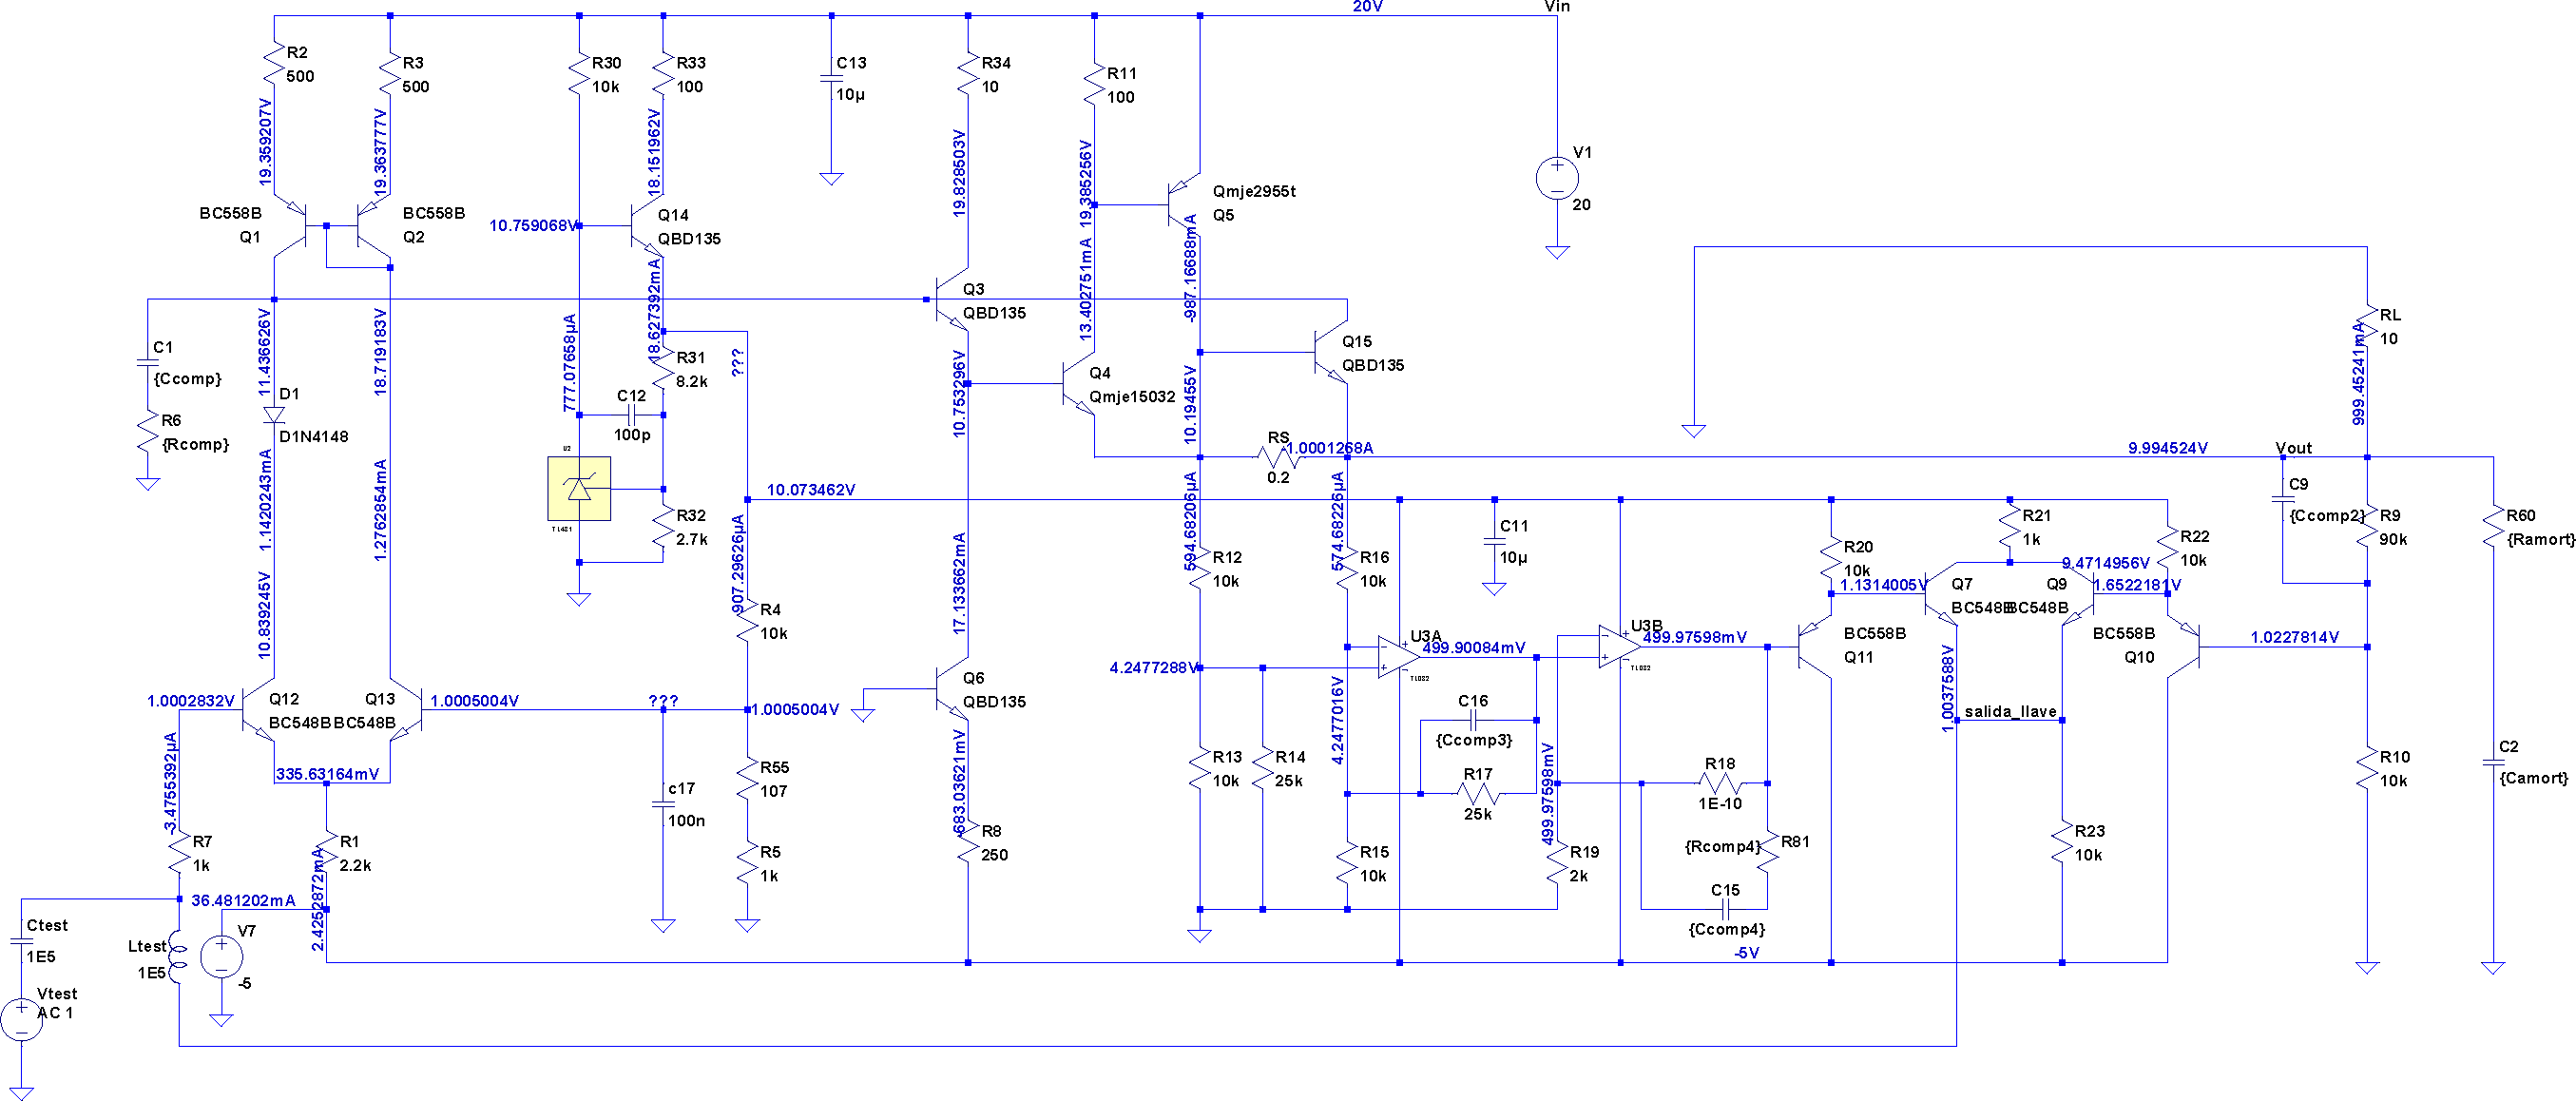
\includegraphics[width=1.2 \textwidth, angle=90]{./img/desarrollo/power_supply_LOOP.png}
\caption{\label{fig:fig_complete_circuit_loop}\footnotesize{Circuito utilizado para la obtención de la ganancia de lazo en función de la frecuencia.}}
\end{center}
\end{figure}

\clearpage

\begin{figure}[H] %htb
\begin{center}
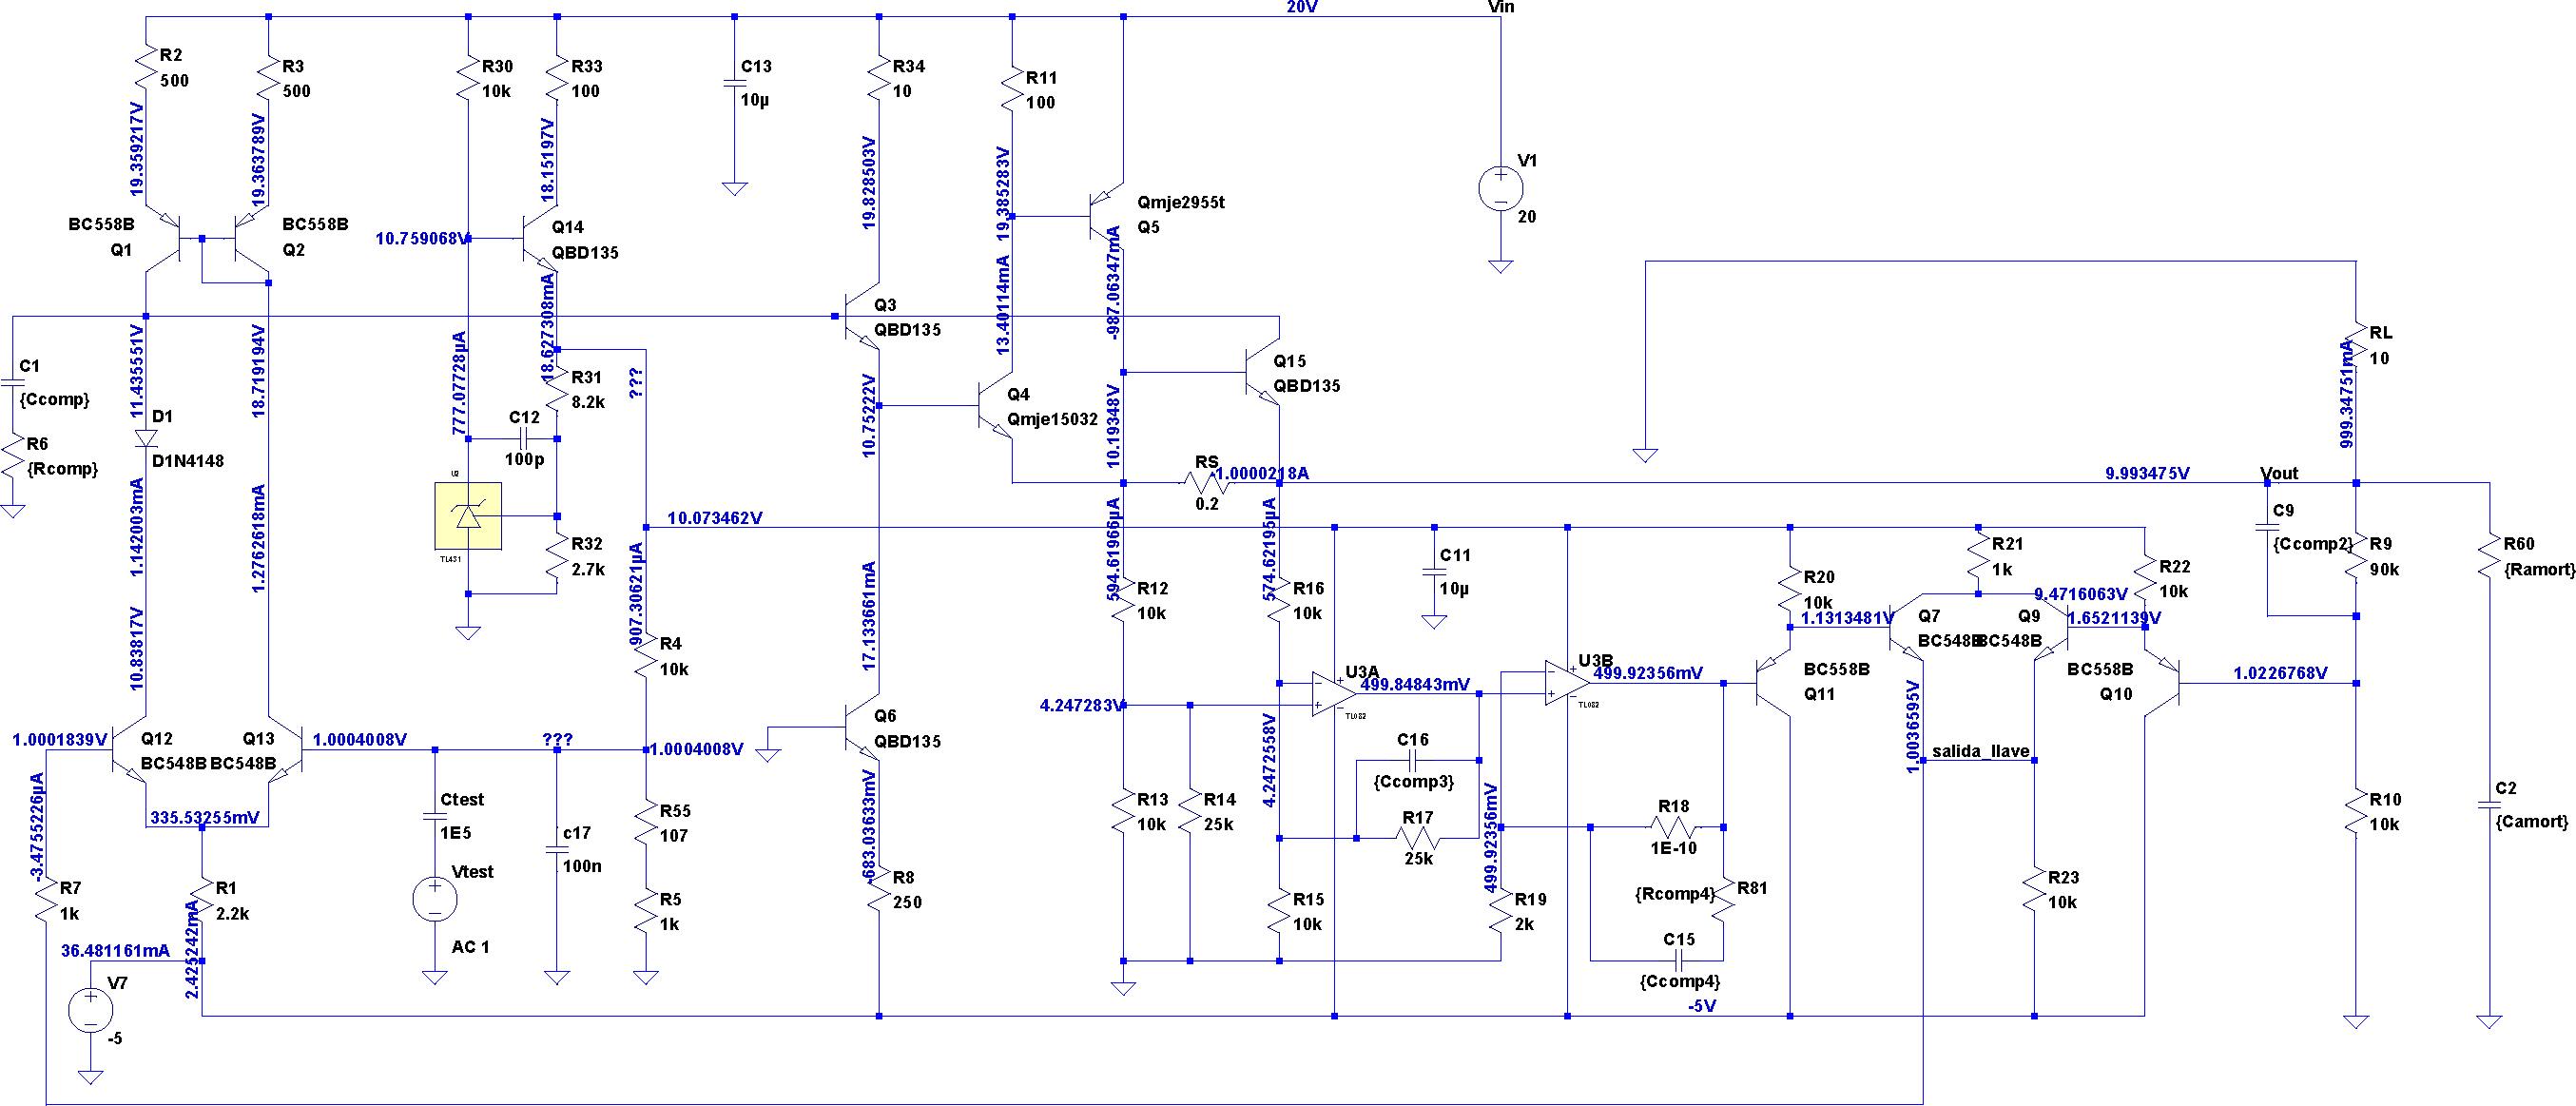
\includegraphics[width=1.2 \textwidth, angle=90]{./img/desarrollo/power_supply_RF.png}
\caption{\label{fig:fig_complete_circuit_rf}\footnotesize{Circuito utilizado para la obtención de la respuesta en frecuencia.}}
\end{center}
\end{figure}

\clearpage

\begin{figure}[H] %htb
\begin{center}
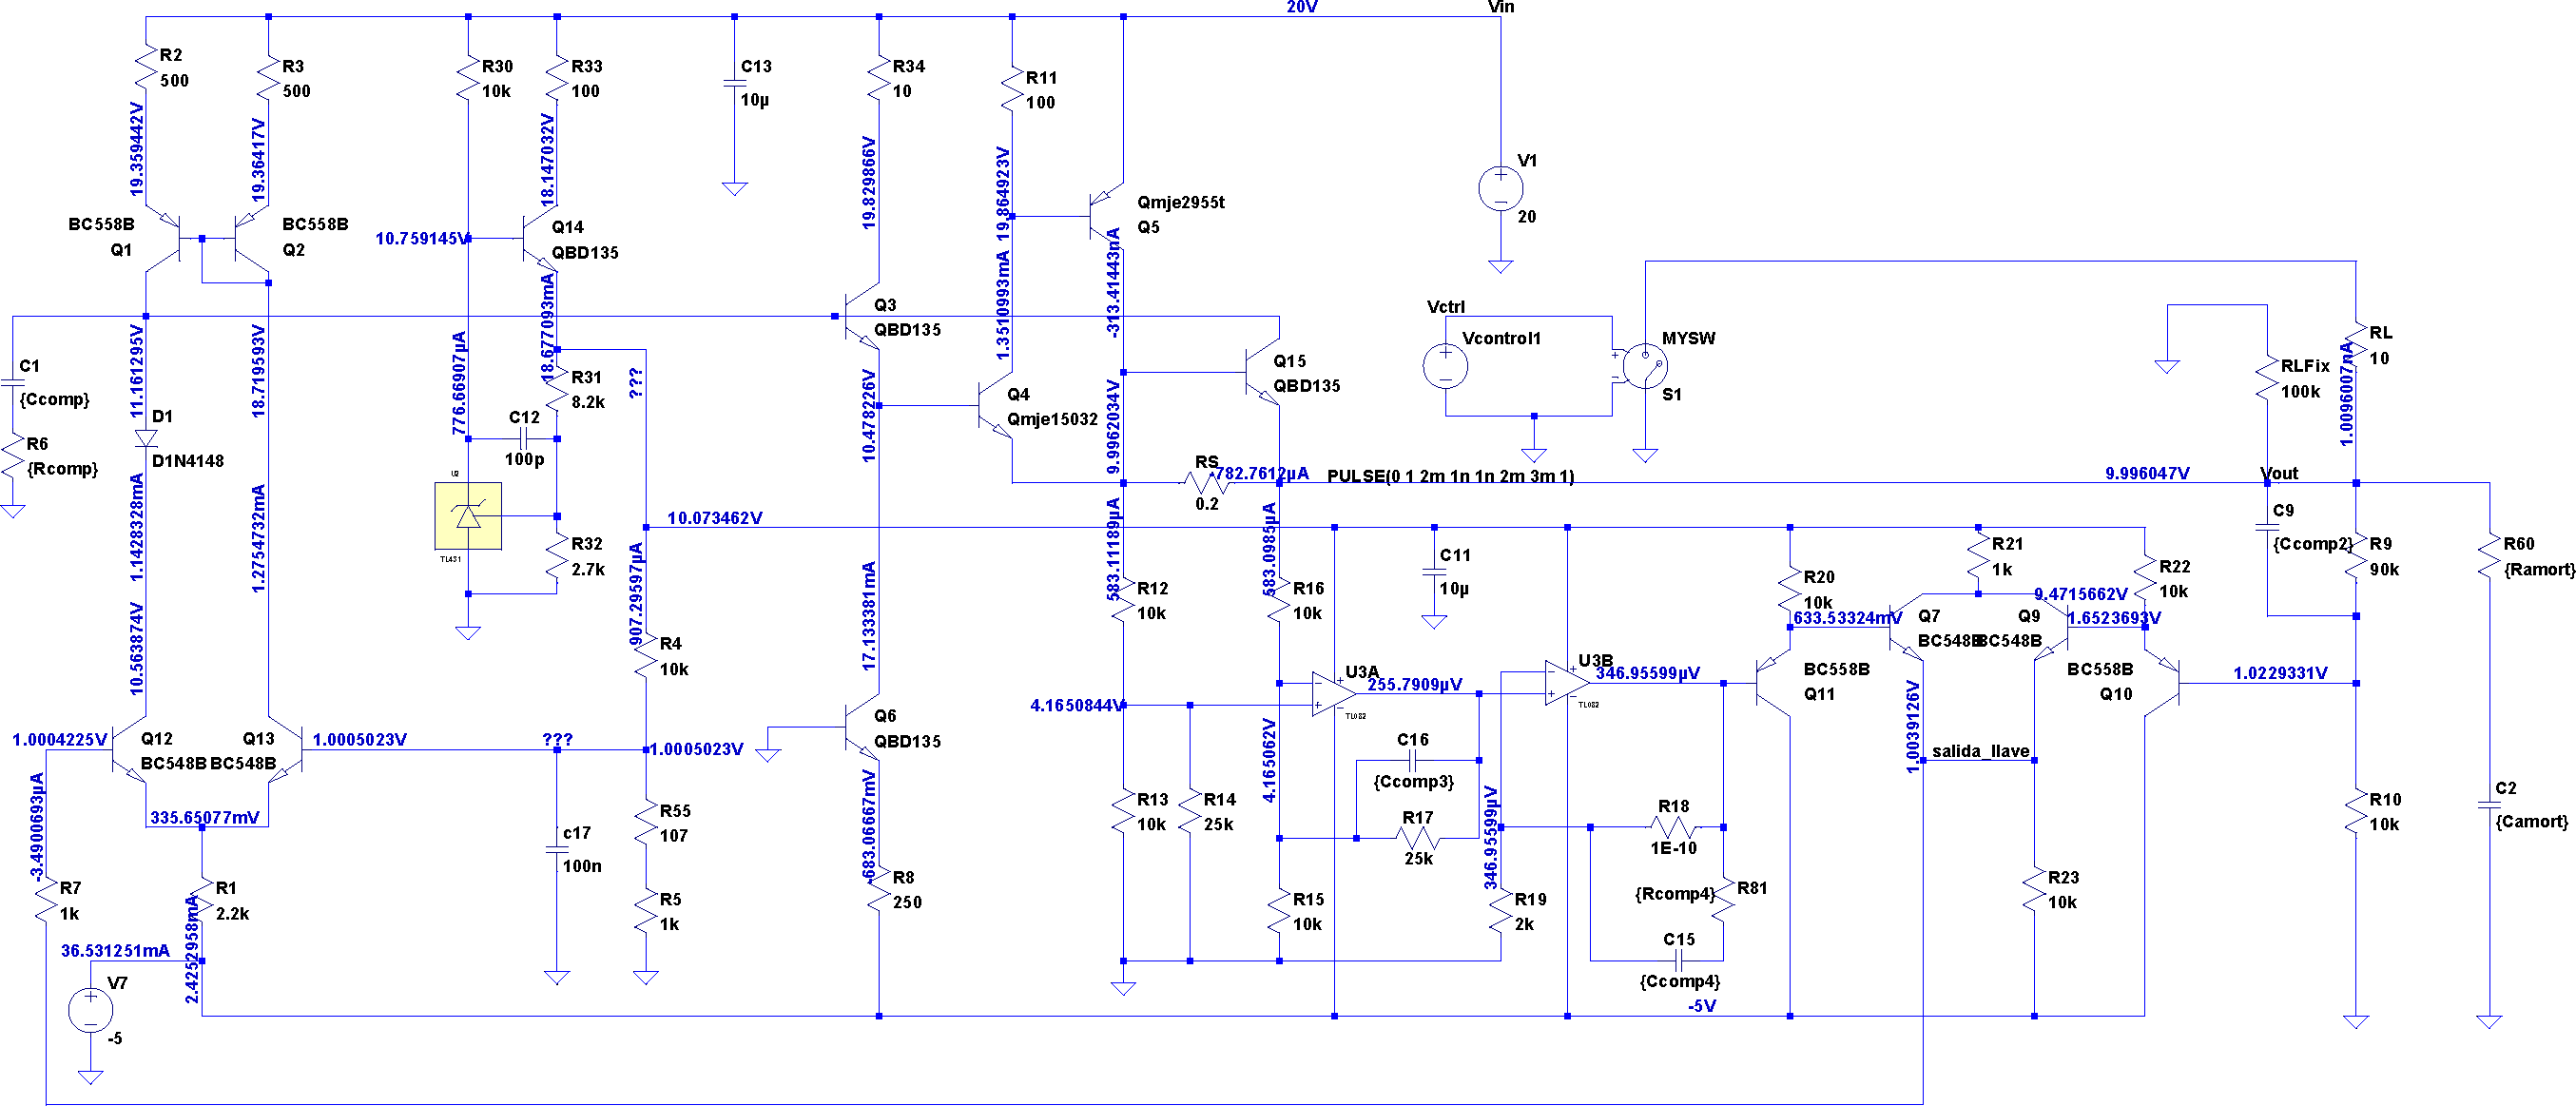
\includegraphics[width=1.2 \textwidth, angle=90]{./img/desarrollo/power_supply_STEP.png}
\caption{\label{fig:fig_complete_circuit_step}\footnotesize{Circuito utilizado para la obtención de la respuesta dinámica.}}
\end{center}
\end{figure}
\clearpage
%\\\\\\\\\\\\\\\\\\\\\\\\\\\

%\\\\\\\\\\\\\\\\\\\\\\\\\\\
\section{Análisis cualitativo}
\resetallcounters

\subsection{Secciones del circuito}


\normalfont

La topología del circuito corresponde a la de un típico amplificador de potencia de tres etapas realimentado, donde la \quotemarks{señal} a amplificar es una referencia de tensión, armada en torno a una referencia de tensión comercial, el \textbf{TL431}, la tensión de salida es muestreada y sumada a la entrada, formando un lazo de realimentación \textbf{serie-paralelo}, estabilizando la tensión de salida, el resultado de esta configuración es una fuente de tensión regulada. El circuito además posee un segundo lazo de realimentación, donde se muestrea la corriente de salida, se convierte a tensión y se suma a la entrada, formando un lazo de realimentación \textbf{serie-serie}, estabilizando la corriente de salida. El circuito trabaja con solo uno de los lazos de realimentación funcionando en un dado momento, el switcheo de uno a otro, se realiza en forma automática, con un subcircuito dedicado, según sea el estado de carga, el amplificador de potencia es el mismo en ambos lazos, solo cambia la red de realimentación. El circuito además cuenta con una limitación extra de corriente que actúa únicamente durante transitorios, además el circuito se encuentra compensado en frecuencia en ambos lazos (tema de la segunda parte del trabajo práctico).
En el circuito se pueden diferenciar claramente las secciones que se marcan en la figura~\figref{fig:fig_complete_circuit_secions}, las mismas son:


\begin{itemize}
\item Amplificador diferencial con caga activa: realiza la suma (resta) de la señal realimentada y provee amplificación.
\item Referencia de tensión: Provee una tensión estable de referencia de aproximadamente $1 \si[per-mode=symbol]{\volt}$ y además provee alimentación para algunas partes del circuito ($10 \si[per-mode=symbol]{\volt}$).
\item Seguidor con carga activa: Provee adaptación de impedancia entre la primera y la tercera etapa.
\item Par compuesto (Sziklai): Maneja la corriente de salida, presentando a la carga una muy baja impedancia y una alta impedancia a la segunda etapa.
\item Limitación de corriente simple: Formada solo por un transistor que limita durante transitorios, simplemente deriva corriente de la base del seguidor (segunda etapa).
\item Llave analógica: Hace el switcheo automático entre los lazos de tensión y corriente, es prácticamente transparente a fines prácticos.
\item Realimentación de tensión: Red de muestreo y realimentación de tensión (la mitad de la llave forma parte de la misma).
\item Realimentación de corriente: Red de muestreo y realimentación de corriente (la mitad de la llave forma parte de la misma).
\end{itemize}


\clearpage
%\\\\\\\\\\\\\\\\\\\\\\\\\\\

%\\\\\\\\\\\\\\\\\\\\\\\\\\\
\section{Análisis por simulación d las redes de compensación}
\resetallcounters

A continuación se analizan cada una de las redes de compensación en los modos correspondientes usando las simulaciones obtenidas para los modos correspondientes indicados en el cuadro~\tableref{table:compensation_networks}, usando los circuitos mostrados en la figura~\figref{fig:fig_complete_circuit_loop}, la figura~\figref{fig:fig_complete_circuit_rf} y la figura~\figref{fig:fig_complete_circuit_step}.\\

Los estados simulados para los casos de modo de regulación de tensión, son:

\begin{itemize}
\item $10 \si[per-mode=symbol]{\volt}$ de salida para $R_{L} = 10 \si[per-mode=symbol]{\ohm}$, $1 \si[per-mode=symbol]{\ampere}$ de carga.

\item $1 \si[per-mode=symbol]{\volt}$ de salida para $R_{L} = 1 \si[per-mode=symbol]{\ohm}$, $1 \si[per-mode=symbol]{\ampere}$ de carga.
\end{itemize}

y los estados simulados para los casos de modo de regulación de corriente, son:

\begin{itemize}
\item $2 \si[per-mode=symbol]{\ampere}$ de salida para $R_{L} = 0 \si[per-mode=symbol]{\ohm}$ (cortocircuito).

\item $200 \si[per-mode=symbol]{\milli\ampere}$ de salida para $R_{L} = 0 \si[per-mode=symbol]{\ohm}$ (cortocircuito).
\end{itemize}



Los modos elegidos responden a ser los casos extremos en modo tensión y modo corriente, de esa manera se espera tener cubierto el espectro de posibles estados de funcionamiento de la fuente de alimentación.\\

Los valores de los componentes de las redes de compensación se analizan para el valor de diseño y dos valores mas, uno por debajo y otro por arriba, tratando de ver porque el valor de diseño es el mas adecuado.\\

El análisis primero consiste en evaluar la simulación de ganancia de lazo en función de la frecuencia, realizando un barrido de frecuencia con el comando \textbf{SPICE} \textit{.ac} y en forma paramétrica con los valores a comparar de las redes de compensación de a uno por vez, para obtener en cada estado los márgenes de fase y de ganancia como se describió en la sección~\sectref{sect_margins_explanation}. En esto cabe aclarar que el análisis es aproximado dado que los márgenes en algunos casos pueden no ser sufientes para garantizar la estabilidad, siendo necesarios para un análisis completo, diagramas de \textbf{Nyquist} y de \textbf{Root Locus}, sin embargo para esto sería necesario un análisis teórico completo que permita obtener las transferencias completas cosa que no corresponde al simple análisis de validación por simulación.\\

Luego también se observa la respuesta en frecuencia del circuito, realizando también un barrido de frecuencia con el comando \textbf{SPICE} \textit{.ac} y en forma paramétrica con los valores a comparar de las redes de compensación de a uno por vez, de esta simulación se obtiene principalmente el ancho de banda del circuito.\\

Finalmente se observa la simulación de la respuesta del circuito a un salto de carga, según el modo analizado, para cada uno de los valores de cada uno de los componentes de las redes de compensación, esto equivale a una respuesta al escalón para este circuito, donde se puede ver si la respuesta es la esperada para un circuito estable, y evaluar si los sobre-picos presentes y el tiempo de crecimiento son aceptables.\\

El análisis se realizará comparando lo obtenido y comentando en cada caso lo mas importante, refiriendo al gráfico relevante.\\

Hay algunos modos que no se analizan por que no aplican, como ser por ejemplo la \textbf{Red~número~4} en el caso de que $R_{18} = 0 \si[per-mode=symbol]{\ohm}$, $I_{out} = 2 \si[per-mode=symbol]{\ampere}$ ,o la \textbf{Red~número~2} cuando $R_{9} = 0 \si[per-mode=symbol]{\ohm}$, $V_{out} = 1 \si[per-mode=symbol]{\volt}$.





\clearpage


%\\\\\\\\\\\\\\\\\\\\\\\\\\\
\subsection{Red de compensación Ccomp/Rcomp}

La red formada por \textbf{Ccomp} y \textbf{Rcomp} actúa tanto para el lazo de tensión como para el de corriente, por lo que se analizan ambos modos.



\subsubsection{Variación de la ganancia de lazo con Ccomp en modo tensión}



\begin{figure}[H] %htb
\begin{center}
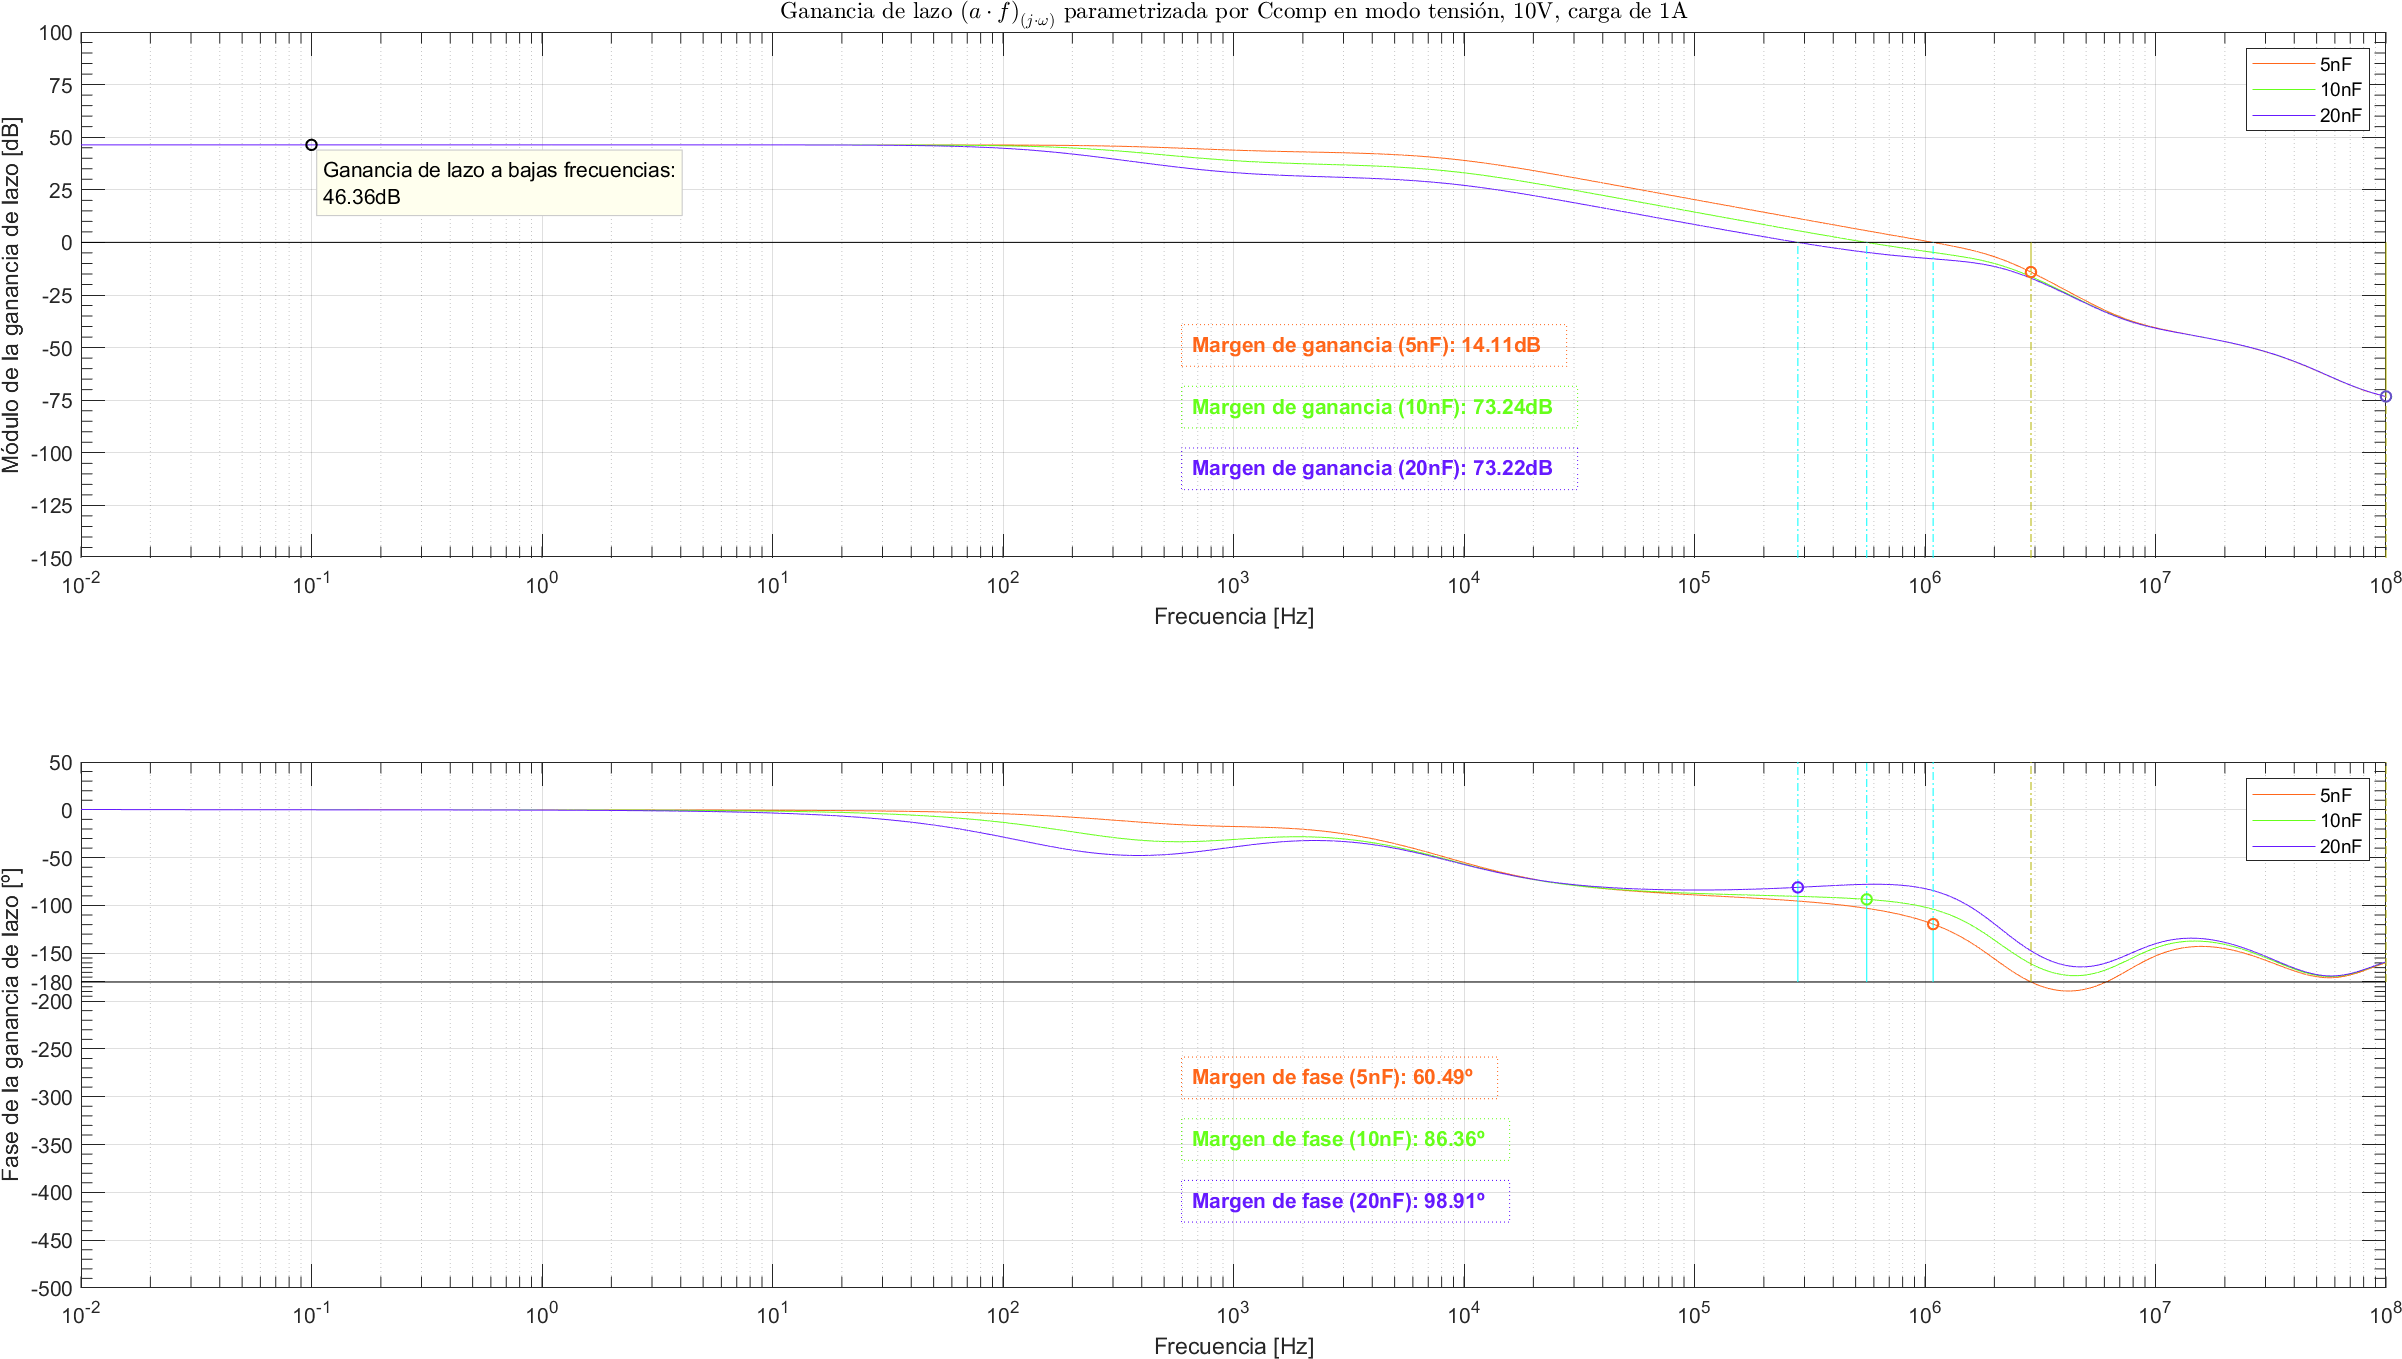
\includegraphics[width=1.1 \textwidth, angle=90]{./img/plots/loop/power_supply_CCOMP_LOOP_Modo1.png}
\caption{\label{fig:fig_power_supply_CCOMP_LOOP_Modo1}\footnotesize{Ganancia de lazo en función de la frecuencia parametrizada por Ccomp.}}
\end{center}
\end{figure}

\clearpage


\clearpage
%\\\\\\\\\\\\\\\\\\\\\\\\\\\





\clearpage
%\\\\\\\\\\\\\\\\\\\\\\\\\\\


%\\\\\\\\\\\\\\\\\\\\\\\\\\\


%\\\\\\\\\\\\\\\\\\\\\\\\\\\
%\section{Respuestas a preguntas en el enunciado}
%\resetallcounters
%
\subsection{Punto 1}

Analizar que función cumple y como opera el subcircuito compuesto por $R_{12}$ a $R_{17}$, $C_{16}$ y $U_{3}A$. Luego incluir $R_{S}$. ¿Qué características tiene éste subcircuito, por ejemplo, su transferencia, su ancho de banda, su dependencia de las especificaciones del amplificador operacional $TL082$, de sus fuentes de alimentación, de la temperatura, de la tolerancia y tecnología de los resistores con los que se lo implemente, etc.


\subsection{Punto 2}

 Analizar qué función cumple y como opera el subcircuito compuesto por $R_{18}$ a $R_{19}$, $C_{15}$ y $U_{3}B$. ¿Qué características tiene éste subcircuito, por ejemplo, su transferencia, su ancho de banda, su dependencia de las especificaciones del amplificador operacional $TL082$, de sus fuentes de alimentación, de la temperatura, de la tolerancia y tecnología de los resistores con lo que se lo implemente, etc. ($R_{18}$ puede variarse desde $0 \Omega$ a $18 K\Omega$).


\subsection{Punto 3}

Analizar qué función cumple y cómo opera el subcircuito compuesto por $R_{20}$ a $R_{23}$ y $Q_{7}$-$Q_{9}$-$Q_{10}$-$Q_{11}$. ¿Qué características tiene éste subcircuito?


\subsection{Punto 4}

Analizar el subcircuito que proporciona la tensión de referencia. ¿Cómo funciona y qué características tiene? Por ejemplo: hallar por cálculo y por simulación el valor de la tensión de referencia y su dependencia de la variación de la tensión de entrada $V_{1}$, de la temperatura ambiente y de la corriente que pueda entregar éste subcircuito a otros subcircuitos que alimente. Consultar las hojas de datos de todos sus componentes, en especial el $TL431$.


\subsection{Punto 5}

Analizar el subcircuito compuesto por $Q_{4}$ y $Q_{5}$. Por ejemplo: con que nombre es conocida su topología, comprobar si es una topología que emplea realimentación, qué características funcionales tiene este subcircuito, que valores de impedancia presente a los otros circuitos que alimente, cual es la transferencia de este subcircuito (variable de salida / variable de entrada), cuál es su ancho de banda, etc.


\subsection{Punto 6}

¿Cuál es el rango de la tensión de salida de la fuente considerando que $R_{9}$ puede variar desde $0 \Omega$ a $90 K\Omega$? (Tomar $R_{L} = 1M\Omega$)


\subsection{Punto 7}

¿Cuál es el rango la corriente de salida de la fuente considerando que $R_{18}$ puede variar desde $0 \Omega$ a $18 K\Omega$? (Tomar $R_{L} = 0\Omega$)


\subsection{Punto 8}

¿Cuál es el valor de la resistencia de carga $R_{L}$ que impone el límite entre el modo fuente de tensión y fuente de corriente para $R_{9} = 90 K\Omega$ y $R_{18} = 0 \Omega$?


\subsection{Punto 9}

¿Qué hace (o para que está) cada componente, o sea, que función cumple en el circuito y justificar el valor de cada resistencia, diodo, transistor, etc?\\
En particular, respecto de la pregunta anterior, explicar que función realiza $D_{1}$ y justificar la elección de su designación como $1N4148$.


\subsection{Punto 10}

¿Qué tecnología, tolerancia, capacidad de disipación de potencia, estabilidad con la temperatura, tensión y corriente de operación máxima y pulsante, características mecánicas, apartamiento de su valor nominal por envejecimiento, etc, debe tener cada componente considerando una implementación física de éste circuito?


\subsection{Punto 11}

Calcular la ganancia de lazo \quotemarks{af} para el lazo de tensión y para el lazo de corriente, comparando en ambos casos con respecto a 1, o sea, ¿resulta af mucho mayor que $1$? Considerar esto para frecuencias del orden de entre $0 Hz$ y $100 Hz$.


\subsection{Punto 12}

Calcular la impedancia de salida, o más propiamente la impedancia en el nodo de salida, para una carga de $100 \Omega$ y una frecuencia en el entorno a $50Hz$. Utilizar para el cálculo los mismo modelos utilizados en la pregunta anterior.


\subsection{Punto 13}

Hallar por simulación la impedancia del nodo de salida en función de la frecuencia para frecuencias desde $0,1 Hz$ hasta $100 KHz$ y con $R_{L} = 100 \Omega$. Considerar $R_{9} = 10 K\Omega$.


\subsection{Punto 14}

Hallar por simulación la impedancia de la malla de salida en función de la frecuencia para frecuencias desde $0,1 Hz$ hasta $100 KHz$ y con  $R_{L} = 0 \Omega$. Considerar  $R_{18} = 0 \Omega$.


\subsection{Punto 15}

Hallar por simulación la tensión del nodo de salida en función de la corriente de salida para  $R_{L}$ variando entre  $100 \Omega$ y $0 \Omega$. Considerar $R_{9} = 10 K\Omega$ y $R_{18} = 0 \Omega$


\subsection{Punto 16}

Hallar por simulación la variación de la tensión de salida en función del tiempo para un salto abrupto de la corriente de salida desde aproximadamente $0 A$ hasta $ 1A$ y posteriormente un salto abrupto de la corriente de salida desde aproximadamente $ 1A$ hasta $0 A$. Considerar $R_{9} = 10 K\Omega$ y $R_{18} = 0 \Omega$.


\subsection{Punto 17}

Calcular la eficiencia para $V_{1}$ igual a $15 V$, $20 V$ y $25 V$ 

\begin{enumerate}
\item[a)] con $R_{L} = 10 \Omega$, $R_{9} = 90 K\Omega$ y $R_{18} = 0 \Omega$
\item[b)] con $R_{L} = 1 \Omega$, $R_{9} = 0 \Omega$ y $R_{18} = 0 \Omega$
\end{enumerate}


\subsection{Punto 18}

¿Cómo influye en la tensión de salida la variación de la fuente de entrada $V_{1}$ (variando de $1 V$ a $30 V$ y con $R_{L} = 10 \Omega$, $R_{9} = 90 K\Omega$ y $R_{18} = 0 \Omega$)? Simular para graficar la tensión de salida en función de $V_{1}$


\subsection{Punto 19}

¿Cómo influye en la corriente de salida la variación de la fuente de entrada $V_{1}$ (variando de $1 V$ a $30 V$ y con $R_{L} = 0 \Omega$, $R_{9} = 90 K\Omega$ y $R_{18} = 0 \Omega$? Simular para graficar la corriente de salida en función de $V_{1}$


\subsection{Punto 20}

Determinar el rechazo de ruido, o sea, ¿Cuántos decibles de diferencia se miden comparando un ruido presente en la tensión de entrada V1 respecto del residuo de ese ruido en la tensión de salida. Debe intentarse no considerar el ruido propio de la fuente. \textbf{NOTA}: el ruido podría ser por ejemplo el rizado resultante de una rectificación y filtrado.


\subsection{Punto 21}

Modificar el circuito de la fuente reemplazando en parte o totalmente el amplificador por el regulador integrado $LM723$ y evaluar el comportamiento del nuevo diseño comparándolo con el original.





%\clearpage
%\\\\\\\\\\\\\\\\\\\\\\\\\\\


%\\\\\\\\\\\\\\\\\\\\\\\\\\\
\section{Observaciones y conclusiones}
\resetallcounters

\subsection{Observaciones y conclusiones}

Cuando empezamos el desarrollo del trabajo práctico intentamos desarrollarlo como si diseñáramos la compensación desde cero, a pesar de que las redes que concluimos que serían necesarias coincidían en la localización con las existentes en el diseño, nos encontramos que el cálculo de los valores requería un desarrollo teórico extenso y una validación iterativa por simulación que se hacia muy complicada en el tiempo disponible, no obstante este primer intento nos sirvió para entender que involucra el diseño de una compensación. \\
Otra cosa en el desarrollo del análisis por simulación es que nos costó un poco en algunos casos ver porque un valor es mejor que otro, al menos por lo que se podía ver en las simulaciones, eso puede ser porque faltan casos que simular, pero ya era bastante extenso como para hacer mas simulaciones. \\
Finalmente, viendo lo justa que queda la compensación para algunos casos, llegamos a la conclusión que sería necesario un análisis por el \textbf{método de Monte Carlo} para garantizar la estabilidad frente a las variaciones de los valores de los componentes, pero nuevamente, el análisis sería demasiado extenso, especialmente dado el tiempo que una simulación estadística puede tomar.
\cleardoublepage
%\\\\\\\\\\\\\\\\\\\\\\\\\\\


%\\\\\\\\\\\\\\\\\\\\\\\\\\\
%Reinicio la cuenta y seteo el estilo de headers y footers.
\pagestyle{bibliostyle}
%\\\\\\\\\\\\\\\\\\\\\\\\\\\

%\\\\\\\\\\\\\\\\\\\\\\\\\\\
\section{Bibliografía}
\resetallcounters

\begin{thebibliography}{9}




\bibitem{Gray_Meyer3}
\Needspace*{7\baselineskip}
\emph{Analysis and Design of Analog Integrated Circuits (3\textsuperscript{rd} Edition)}\\
Author: Paul R. Gray\\
Author: Robert G. Meyer\\
Publisher: John Wiley \& Sons, Inc.; 3\textsuperscript{rd} Edition (Janury 15, 1993)\\
Copyright: \textcopyright \space 1993, John Wiley \& Sons, Inc.\\
ISBN 10: 0471574953\\
Website: \weblink{http://www.wiley.com/WileyCDA/WileyTitle/productCd-EHEP000220.html}{Analysis and Design of Analog Integrated Circuits (3\textsuperscript{rd} Edition)}\\




\bibitem{Gray_Meyer4}
\Needspace*{10\baselineskip}
\emph{Analysis and Design of Analog Integrated Circuits (4\textsuperscript{th} Edition)}\\
Author: Paul R. Gray\\
Author: Paul J. Hurst\\
Author: Stephen H. Lewis\\
Author: Robert G. Meyer\\
Publisher: John Wiley \& Sons, Inc.; 4\textsuperscript{th} Edition (2001)\\
Copyright: \textcopyright \space 2001, John Wiley \& Sons, Inc.\\
ISBN 10: 0471321680\\
ISBN 13: 9780471321682\\
Website: \weblink{http://www.wiley.com/WileyCDA/WileyTitle/productCd-EHEP000220.html}{Analysis and Design of Analog Integrated Circuits (4\textsuperscript{th} Edition)}\\




\bibitem{Gray_Meyer5}
\Needspace*{10\baselineskip}
\emph{Analysis and Design of Analog Integrated Circuits (5\textsuperscript{th} Edition)}\\
Author: Paul R. Gray\\
Author: Paul J. Hurst\\
Author: Stephen H. Lewis\\
Author: Robert G. Meyer\\
Publisher: John Wiley \& Sons, Inc.; 5\textsuperscript{th} Edition (2009)\\
Copyright: \textcopyright \space 2001, John Wiley \& Sons, Inc.\\
ISBN 10: 0470245999\\
ISBN 13: 9780470245996\\
Website: \weblink{https://www.wiley.com/en-ar/Analysis+and+Design+of+Analog+Integrated+Circuits\%2C+5th+Edition-p-9780470245996}{Analysis and Design of Analog Integrated Circuits (5\textsuperscript{th} Edition)}\\



\bibitem{Sedra_Smith_ESP4}
\Needspace*{9\baselineskip}
\emph{Circuitos microelectrónicos (4\textsuperscript{ta} Edición) español}\\
Author: Adel. S. Sedra\\
Author: Kenneth C. Smith\\
Publisher: Oxford, University press; 4\textsuperscript{ta} Edición (2001)\\
Copyright: \textcopyright \space 1999, Oxford, University press México.\\
Original Copyright: \textcopyright \space 1998, 1991, 1987, 1982, Oxford, University press Inc.\\
ISBN 10: 01951166310\\
Website: \weblink{http://www.oup.com/us/companion.websites/0195142519/}{Circuitos microelectrónicos (4\textsuperscript{ta} Edición) español}\\




\bibitem{Sedra_Smith_ENG5}
\Needspace*{8\baselineskip}
\emph{Microelectronic circuits (5\textsuperscript{th} Edition)}\\
Author: Adel. S. Sedra\\
Author: Kenneth C. Smith\\
Publisher: Oxford, University press; 5\textsuperscript{th} Edition (2004)\\
Copyright: \textcopyright \space 2004, 1998, 1991, 1987, 1982, Oxford, University press Inc.\\
ISBN 10: 0195142527\\
Website: \weblink{http://www.oup.com/us/companion.websites/0195142519/}{Microelectronic circuits (5\textsuperscript{th} Edition)}\\





\end{thebibliography}
\cleardoublepage
%\\\\\\\\\\\\\\\\\\\\\\\\\\\

%\\\\\\\\\\\\\\\\\\\\\\\\\\\
%Seteo el stilo de headers y footers.
\pagestyle{allpages}
%\\\\\\\\\\\\\\\\\\\\\\\\\\\

\appendix


\appendixpage
\addappheadtotoc

%\\\\\\\\\\\\\\\\\\\\\\\\\\\


%\\\\\\\\\\\\\\\\\\\\\\\\\\\
\section{Análisis teórico de subcircuitos}

\resetallcounters
%
\subsection{Amplificadores con operacionales}

\label{section:modelo_operacional}

En esta sección analizamos distintas configuraciones con amplificadores operacionales, pero teniendo en cuenta ciertos aspectos de los amplificadores operacionales reales, en particular usamos un modelo lineal, y lo analizamos a bajas/medias frecuencias, sin tener en cuenta en principio el ancho de banda, ni cosas como el \textit{slew rate}, que corresponden a efectos que no se pueden modelar linealmente. El modelo utilizado es el mostrado en la figura~\figref{fig:fig_operational_non_ideal}, como se puede ver, solo consideramos, una ganancia de tensión diferencial de valor finito, una resistencia de entrada también finita y una resistencia de salida mayor a $0$.

\begin{figure}[H] %htb
\begin{center}
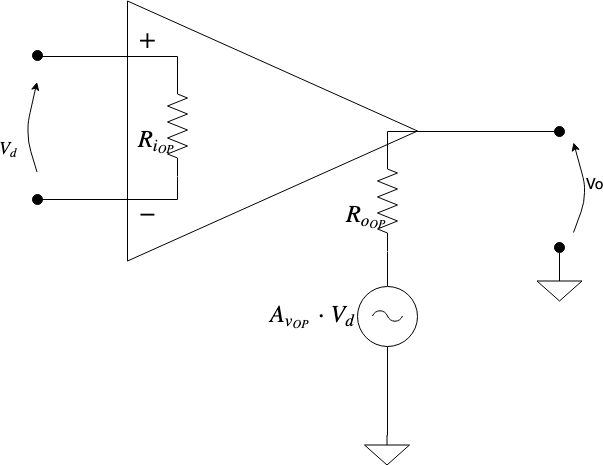
\includegraphics[width=1 \textwidth, angle=0]{./img/operacionales/OP_NONIDEAL_MODEL.png}
\caption{\label{fig:fig_operational_non_ideal}\footnotesize{Modelo lineal de un operacional no ideal.}}
\end{center}
\end{figure}

\vfill

\clearpage

\subsubsection{Amplificador no inversor}

Usando el modelo descripto en la sección~\sectref{section:modelo_operacional} analizamos el circuito mostrado en la figura~\figref{fig:fig_operational_ideal_non_inverter}. El circuito es un amplificador no inversor con amplificador no operacional. El análisis que se hará por realimentación, pretende analizar como es la transferencia de mismo con nuestro modelo, y como influye la no idealidad del operacional en la transferencia, para finalmente ver a que se reduce la transferencia al llevar las expresiones al caso ideal.

\begin{figure}[H] %htb
\begin{center}
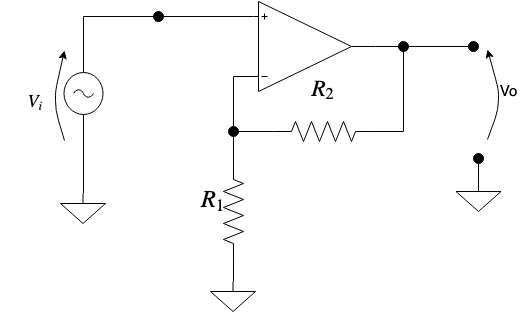
\includegraphics[width=0.5 \textwidth, angle=0]{./img/operacionales/OP_NINV.png}
\caption{\label{fig:fig_operational_ideal_non_inverter}\footnotesize{Amplificador no inversor.}}
\end{center}
\end{figure}




\subsubsection{Amplificador inversor}


\subsubsection{Amplificador diferencial}
%
%\clearpage
%
%
\subsection{Par compuesto (Sziklai)}




%
%\clearpage
%
%
\subsection{Llave electrónica transparente}

\label{section:switch}

El circuito cumple la función de una especie de compuerta OR analógica, poniendo a la salida tanto en el nivel de continua, como en el nivel de señal, el nivel de la terminal de entrada de mayor potencial.\\ 
El nivel de tensión continua a la salida, es prácticamente igual al nivel de tensión continua a la entrada, debido a las tensiones $V_{be}$ compensadas por las dos etapas, habrá una pequeña diferencia dada por las diferencias entre los transistores y diferencias en la corriente de colector.\\
La entrada con mayor potencial eleva el potencial en los emisores de los transistores internos de la llave, $Q_{7}$ y $Q_{8}$, y hace que se corte el transistor de la entrada con menor potencial. \\
Otra cosa importante es que la llave es perfectamente simétrica, si las tensiones de entrada se invierten, los puntos de trabajo de los transistores de cada mitad de la llave se invierten.\\
A los efectos de señal para la terminal de entrada que comande la salida, son dos seguidores en cascada, esto sumado a lo dicho en el párrafo anterior, justifica hablar de una llave trasparente. Otro detalle importante, es que por tratarse de dos seguidores en cascada, se tiene una impedancia muy alta de entrada, cargando muy poco a los circuitos conectados a las entradas.\\
Utilizamos el circuito mostrado en la figura~\figref{fig:fig_analogic_switch}, para simular su comportamiento, utilizando en una de sus entradas un valor de continua fijo, $1 \si[per-mode=symbol]{\volt}$, y una señal cuadrada de $1.1 \si[per-mode=symbol]{\volt}$ de pico y $500 \si[per-mode=symbol]{\hertz}$ en su otra entrada. Se eligió una frecuencia de un valor tal que se puedan observar algunos efectos reactivos en el circuito. Se realizó una simulación de tipo transitorio con el comando \textbf{SPICE} \textit{.tran}, el resultado se exportó y se graficó en \textbf{MATLAB}, el resultado de la simulación se puede ver en la figura~\figref{fig:fig_analogic_switch_simulation}, se puede observar claramente como la salida sigue a la entrada de la llave con mayor potencial, y se pueden observar también los efectos reactivos, mayormente debidos a la discontinuidad de la señal en una de las entradas.\\
En cuanto al ancho de banda del circuito, por tratarse de una cascada de dos seguidores, tendremos que el ancho de banda será seguramente limitado por las bases de los transistores, en particular el transistor exterior que este activo, al tener una gran resistencia de entrada, y si el el circuito de entrada agrega capacidad a este nodo, sin duda será este el nodo limitante, pero si no es el caso y solo influyen las capacidades parásitas de los transistores, se puede esperar un ancho de banda de varios $\si[per-mode=symbol]{\mega\hertz}$, en particular para este circuito sin cargas o entradas capacitivas, realizando una simulación con el comando \texttt{SPICE} \textit{.ac} desde la entrada activa, se obtuvo $36.1 \si[per-mode=symbol]{\mega\hertz}$.


\vfill

\clearpage

\begin{figure}[H] %htb
\begin{center}
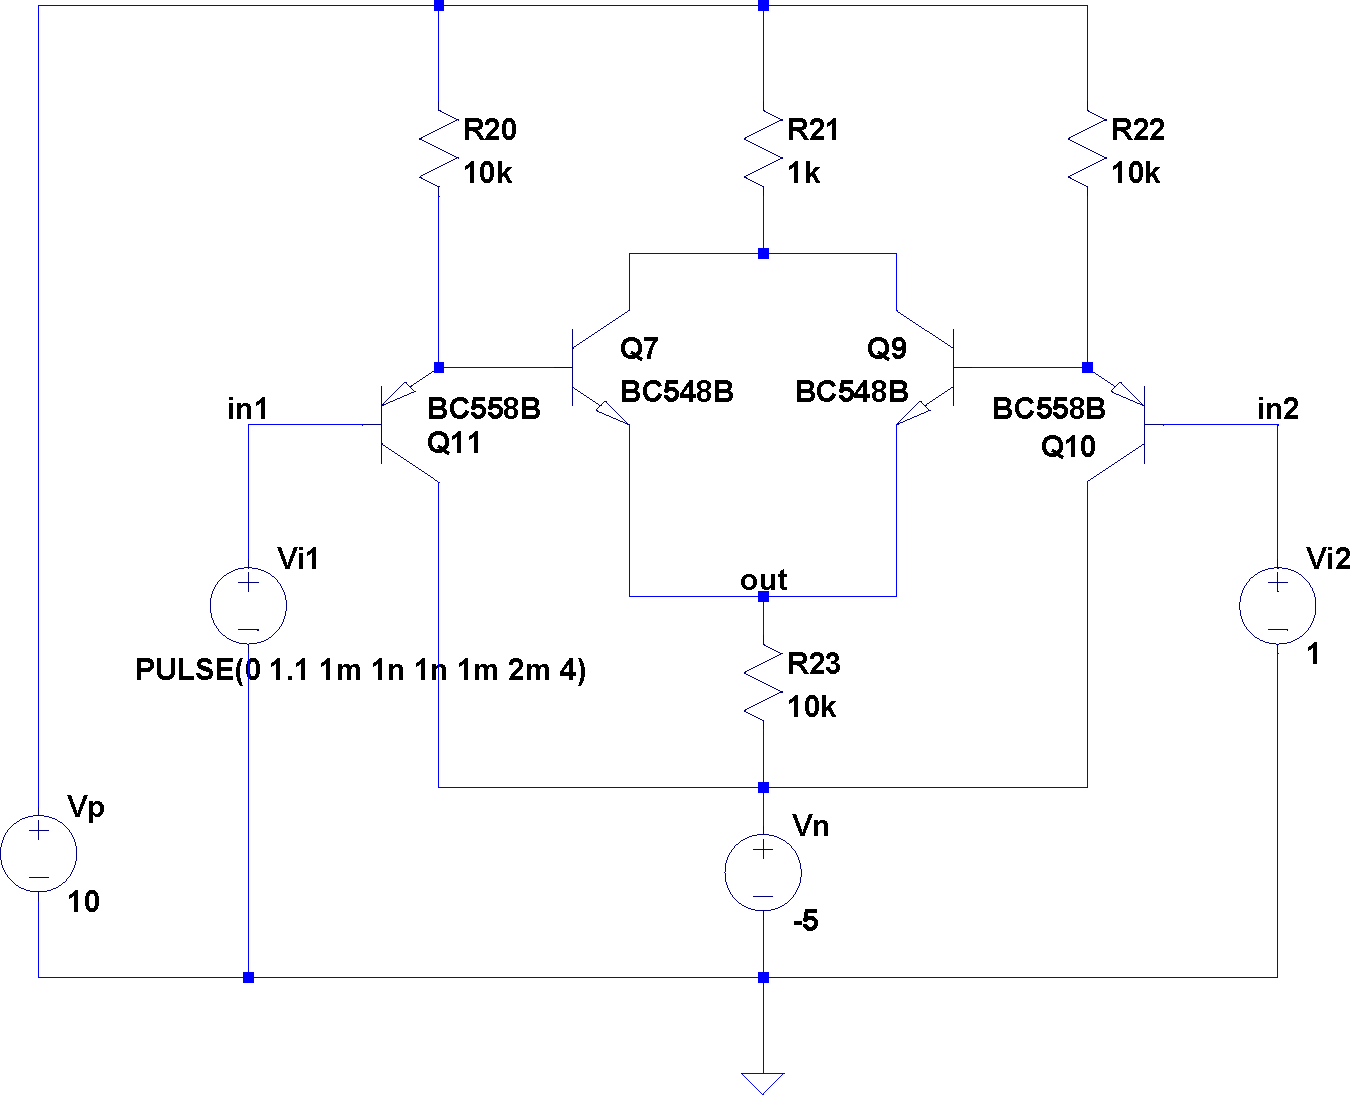
\includegraphics[width=1 \textwidth, angle=0]{./img/llave/OR-Q7-9-10-11.png}
\caption{\label{fig:fig_analogic_switch}\footnotesize{Circuito utilizado para simular la llave analógica.}}
\end{center}
\end{figure}

\vfill

\clearpage


\begin{figure}[H] %htb
\begin{center}
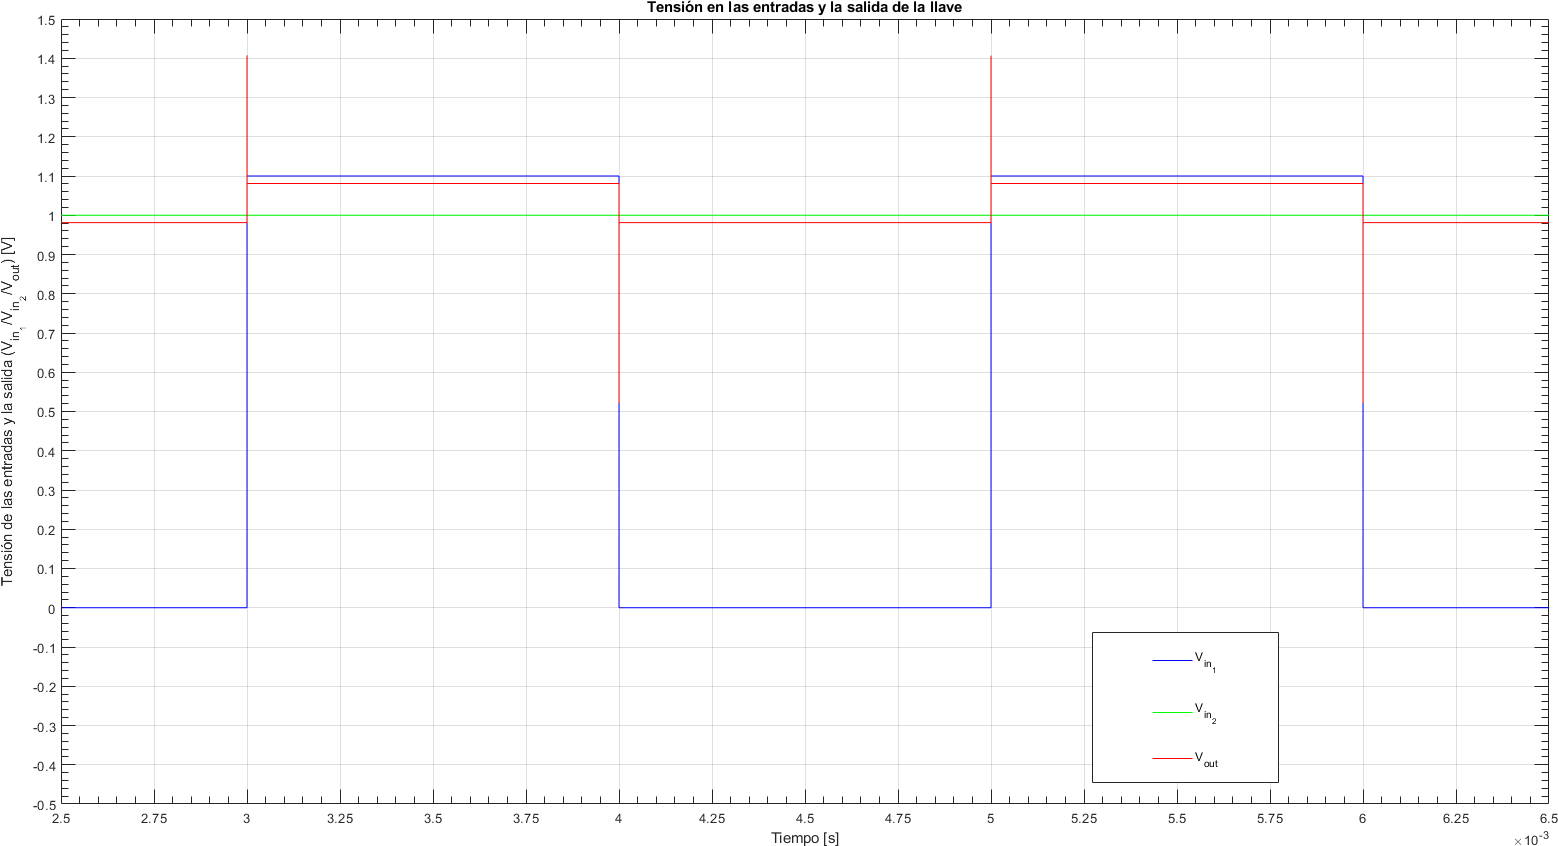
\includegraphics[width=1.2 \textwidth, angle=90]{./img/llave/switch_response.png}
\caption{\label{fig:fig_analogic_switch_simulation}\footnotesize{Respuesta de la llave analógica.}}
\end{center}
\end{figure}

\clearpage
%
%\clearpage
%
%
\subsection{Referencia de tensión basada en el \textit{TL431}}

\label{section:voltage_reference}


\begin{wrapfigure}{rH}{0.18\textwidth}
\begin{center}
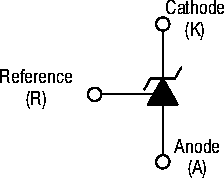
\includegraphics[width=0.15 \textwidth, angle=0]{./img/voltage_reference/reference0.png}
\end{center}
\caption{\label{fig:fig_vref_cir_0}\footnotesize{$TL431$}}
\end{wrapfigure}


Se debe analizar un circuito de referencia de tensión, basado en la referencia integrada $TL431$, el cual se trata de un regulador paralelo (shunt regulator) programable, que opera básicamente como un zener configurable, (su símbolo es similar, como se muestra en la figura~\figref{fig:fig_vref_cir_0}), de bajo coeficiente térmico y bajo ruido, puede ser configurado para tensiones de salida desde el valor de la referencia interna, $V_{ref} = 2.5 \si[per-mode=symbol]{\volt}$, hasta $36 \si[per-mode=symbol]{\volt}$, no tiene un valor per se de tensión de \quotemarks{dropout}, pero por supuesto es necesario que la tensión de entrada sea mayor que la de salida, al tiempo que es polarizado con una corriente de al menos $1 \si[per-mode=symbol]{\milli\ampere}$, lo que impone indirectamente el valor mínimo de tensión de entrada.
La referencia tiene capacidad de absorber desde $1 \si[per-mode=symbol]{\milli\ampere}$ a $100 \si[per-mode=symbol]{\milli\ampere}$ y tiene típicamente una impedancia dinámica de $220 \si[per-mode=symbol]{\milli\ohm}$. La referencia interna de tensión es del tipo \quotemarks{bandgap reference}, que como se explica en el libro G\&M~\cite{Gray_Meyer5}, logra una tensión independiente de la temperatura. Si se tiene en cuenta el esquema simplificado del circuito proveído por el fabricante, que se puede ver el la figura~\figref{fig:fig_vref_cir_2}, se hace mas simple ver la estructura del circuito que se propone analizar, el mismo se puede ver en la figura~\figref{fig:fig_vref_cir_1}. La estructura corresponde al de una fuente de tensión regulada realimentada serie, el elemento de paso es el transistor, $Q_{1}$ en ese diagrama, los resistores, $R_{1}$ y $R_{2}$, son la red de realimentación, que muestrean la tensión de salida y el amplificador suma (resta) en la entrada, teniéndose realimentación del tipo \textbf{serie-paralelo}, que estabiliza la ganancia de tensión, el resistor $R_{3}$ es el que provee la corriente de polarización al $TL431$ y $R_{4}$ está limitando la corriente de colector máxima que puede circular por $Q_{1}$. Interpretado de esta manera es fácil deducir la expresión de cálculo que el fabricante provee para la tensión de salida, ya que, asumiendo que la ganancia del amplificador interno es lo suficientemente elevada como para que la ganancia de lazo sea mucho mayor a $1$, sabemos que la ganancia a lazo cerrado será $\frac{1}{f}$, y es fácil ver que se tiene $f = \frac{R_{2}}{R_{1} + R_{2}}$, por lo tanto la salida que se tendrá será $V_{o} = V_{ref} \cdot \left(1 +  \frac{R_{1}}{R_{2}} \right)$, que salvo por la corrección por la corriente que toma el amplificador, coincide con la proveída. Queda el capacitor $C_{1}$, este se encuentra conectado de manera de proveer realimentación del tipo \textbf{paralelo-paralelo}, de un valor creciente con la frecuencia, de modo que está cumpliendo una función de compensación, lo cual era esperable dado que se tiene internamente un amplificador realimentado. Nuestro circuito tendrá una mayor capacidad de manejar corriente, gracias al transistor $Q_{1}$, que al ser un $BD135$, tiene un $\beta$ mínimo de 25, con lo que tomará $25$ veces menos corriente por la base, se espera que el transistor mejore la resistencia dinámica del $TL431$, ya que se tendrá aproximadamente $r_{d}$ del transistor dividida por la ganancia de lazo, se realizó una simulación con el comando \textbf{SPICE} \textit{.ac}, usando una fuente de corriente de señal a la salida del circuito, para obtener la impedancia de salida, se obtuvo para este circuito $11 \si[per-mode=symbol]{\milli\ohm}$.
El modelo que provee el fabricante es un macro-modelo, que por supuesto no simula todos los detalles del comportamiento, en particular la hojas de datos especifica que la mínima corriente de cátodo para regulaciión es minimamente $1 \si[per-mode=symbol]{\milli\ampere}$ y típicamente $500 \si[per-mode=symbol]{\micro\ampere}$, sin embargo la simulación muestra que regula con corrientes mucho menores, por lo tanto para determinar la máxima corriente que el circuito puede entregar se todo el valor mínimo de corriente de cátodo, $500 \si[per-mode=symbol]{\micro\ampere}$, como limitante y se determinó un valor de corriente de salida, tal que provoque que la base del transistor tome una corriente tal que lleve la de cátodo a ese valor, y se obtuvo $50.4 \si[per-mode=symbol]{\milli\ampere}$.La estabilidad con la temperatura del circuito debería ser similar a la del $TL431$, que es de $40 ppm/^{\circ}C$.



\begin{figure}[H] %htb
\begin{center}
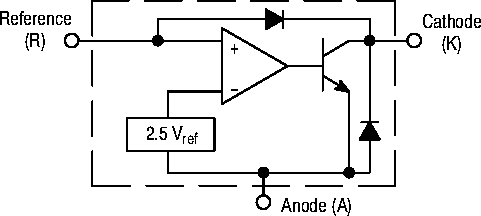
\includegraphics[width=0.65 \textwidth, angle=0]{./img/voltage_reference/reference2.png}
\end{center}
\caption{\label{fig:fig_vref_cir_2}\footnotesize{Esquema interno simplificado del $TL431$}}
\end{figure}



\begin{figure}[H] %htb
\begin{center}
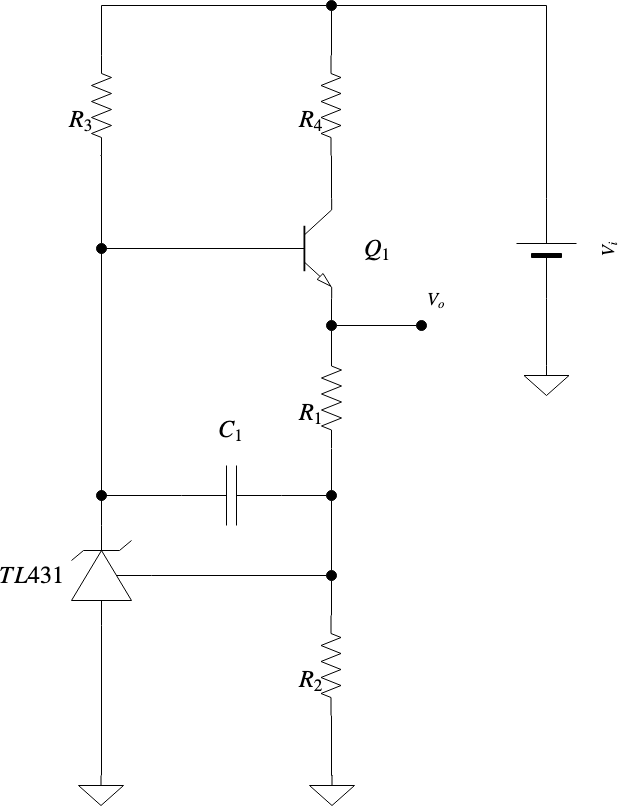
\includegraphics[width=0.50 \textwidth, angle=0]{./img/voltage_reference/reference1.png}
\caption{\label{fig:fig_vref_cir_1}\footnotesize{Circuito de referencia de tensión analizado}}
\end{center}
\end{figure}



\clearpage

%\\\\\\\\\\\\\\\\\\\\\\\\\\\


%\\\\\\\\\\\\\\\\\\\\\\\\\\\


%\\\\\\\\\\\\\\\\\\\\\\\\\\\

\section{Hojas de datos}



%*********************************************

\subsection{TL431}
\label{datasheet_TL431}
\emph{\textbf{TL431}}\\
\emph{Adjustable precision shunt regulator}\\
\vspace{5pt}
Manufacturer page:	\weblink{http://www.ti.com/product/TL431}{http://www.ti.com/product/TL431}\\

Manufacturer Datasheet:	\weblink{http://www.ti.com/lit/gpn/tl431}{http://www.ti.com/lit/gpn/tl431}\\


\subsection{TL082}
\label{datasheet_TL082}
\emph{\textbf{TL082}}\\
\emph{Dual High Slew Rate JFET-Input Operational Amplifier}\\
\vspace{5pt}
Manufacturer page:	\weblink{http://www.ti.com/product/TL082?keyMatch=TL082}{http://www.ti.com/product/TL082?keyMatch=TL082}\\

Manufacturer Datasheet:	\weblink{http://www.ti.com/lit/gpn/tl082}{http://www.ti.com/lit/gpn/tl082}\\


\subsection{BC548}
\label{datasheet_BC548}
\emph{\textbf{BC548}}\\
\emph{NPN Epitaxial Silicon Transistor}\\
\vspace{5pt}
Manufacturer page:	\weblink{https://www.onsemi.com/PowerSolutions/product.do?id=BC548}{https://www.onsemi.com/PowerSolutions/product.do?id=BC548}\\

Manufacturer Datasheet:	\weblink{https://www.onsemi.com/pub/Collateral/BC550-D.pdf}{https://www.onsemi.com/pub/Collateral/BC550-D.pdf}\\


\subsection{BC558}
\label{datasheet_BC558}
\emph{\textbf{BC558}}\\
\emph{PNP Bipolar Transistor}\\
\vspace{5pt}
Manufacturer page:	\weblink{https://www.onsemi.com/PowerSolutions/product.do?id=BC558B}{https://www.onsemi.com/PowerSolutions/product.do?id=BC558B}\\

Manufacturer Datasheet:	\weblink{https://www.onsemi.com/pub/Collateral/BC556B-D.PDF}{https://www.onsemi.com/pub/Collateral/BC556B-D.PDF}\\

\clearpage


\subsection{BD137}
\label{datasheet_BD137}
\emph{\textbf{BD137}}\\
\emph{$1.5 \si[per-mode=symbol]{\ampere}$, $60 \si[per-mode=symbol]{\volt}$ NPN Bipolar Power Transistor}\\
\vspace{5pt}
Manufacturer page:	\weblink{https://www.onsemi.com/PowerSolutions/product.do?id=BD137}{https://www.onsemi.com/PowerSolutions/product.do?id=BD137}\\

Manufacturer Datasheet:	\weblink{https://www.onsemi.com/pub/Collateral/BD135-D.PDF}{https://www.onsemi.com/pub/Collateral/BD135-D.PDF}\\


\subsection{MJE15032}
\label{datasheet_MJE15032}
\emph{\textbf{MJE15032}}\\
\emph{Bipolar Transistor, NPN, $250 \si[per-mode=symbol]{\volt}$, $8.0 \si[per-mode=symbol]{\ampere}$}\\
\vspace{5pt}
Manufacturer page:	\weblink{https://www.onsemi.com/PowerSolutions/product.do?id=MJE15032}{https://www.onsemi.com/PowerSolutions/product.do?id=MJE15032}\\

Manufacturer Datasheet:	\weblink{https://www.onsemi.com/pub/Collateral/MJE15032-D.PDF}{https://www.onsemi.com/pub/Collateral/MJE15032-D.PDF}\\


\subsection{MJE2955}
\label{datasheet_MJE2955}
\emph{\textbf{MJE2955}}\\
\emph{Bipolar Power Transistor, PNP, $10 \si[per-mode=symbol]{\ampere}$, $60 \si[per-mode=symbol]{\volt}$, $75 \si[per-mode=symbol]{\watt}$}\\
\vspace{5pt}
Manufacturer page:	\weblink{https://www.onsemi.com/PowerSolutions/product.do?id=MJE2955T}{https://www.onsemi.com/PowerSolutions/product.do?id=MJE2955T}\\

Manufacturer Datasheet:	\weblink{https://www.onsemi.com/pub/Collateral/MJE2955T-D.PDF}{hhttps://www.onsemi.com/pub/Collateral/MJE2955T-D.PDF}\\


\subsection{Metal film resistor}
\label{datasheet_METALFILMRESISTOR}
\emph{\textbf{Metal film resistor}}\\
\emph{Metal film resistor}\\
\vspace{5pt}
Manufacturer page:	\weblink{https://www.vishay.com/resistors-fixed/metal-film/tab/doclibrary/}{https://www.vishay.com/resistors-fixed/metal-film/tab/doclibrary/}\\



\subsection{Carbon film resistor}
\label{datasheet_CARBONFILMRESISTOR}
\emph{\textbf{Carbon film resistor}}\\
\emph{Carbon film resistor}\\
\vspace{5pt}
Manufacturer page:	\weblink{http://www.vishay.com/resistors-fixed/carbon-film/tab/doclibrary/}{http://www.vishay.com/resistors-fixed/carbon-film/tab/doclibrary/}\\


\clearpage


\subsection{Ceramic capacitor}
\label{datasheet_CERAMIC_CAPACITOR}
\emph{\textbf{Ceramic capacitor}}\\
\emph{Ceramic disk capacitor}\\
\vspace{5pt}
Manufacturer page:	\weblink{https://www.vishay.com/capacitors/ceramic/disc/}{https://www.vishay.com/capacitors/ceramic/disc/}\\


\subsection{Electrolitic Aluminum capacitor}
\label{datasheet_ELECTROLITIC_CAPACITOR}
\emph{\textbf{Electrolitic capacitor}}\\
\emph{Electrolitic aluminum capacitor}\\
\vspace{5pt}
Manufacturer page:	\weblink{https://www.vishay.com/capacitors/aluminum/}{https://www.vishay.com/capacitors/aluminum/}\\










\clearpage
%\\\\\\\\\\\\\\\\\\\\\\\\\\\

\end{document}
